\documentclass[twoside]{book}

% Packages required by doxygen
\usepackage{fixltx2e}
\usepackage{calc}
\usepackage{doxygen}
\usepackage[export]{adjustbox} % also loads graphicx
\usepackage{graphicx}
\usepackage[utf8]{inputenc}
\usepackage{makeidx}
\usepackage{multicol}
\usepackage{multirow}
\PassOptionsToPackage{warn}{textcomp}
\usepackage{textcomp}
\usepackage[nointegrals]{wasysym}
\usepackage[table]{xcolor}

% Font selection
\usepackage[T1]{fontenc}
\usepackage[scaled=.90]{helvet}
\usepackage{courier}
\usepackage{amssymb}
\usepackage{sectsty}
\renewcommand{\familydefault}{\sfdefault}
\allsectionsfont{%
  \fontseries{bc}\selectfont%
  \color{darkgray}%
}
\renewcommand{\DoxyLabelFont}{%
  \fontseries{bc}\selectfont%
  \color{darkgray}%
}
\newcommand{\+}{\discretionary{\mbox{\scriptsize$\hookleftarrow$}}{}{}}

% Page & text layout
\usepackage{geometry}
\geometry{%
  a4paper,%
  top=2.5cm,%
  bottom=2.5cm,%
  left=2.5cm,%
  right=2.5cm%
}
\tolerance=750
\hfuzz=15pt
\hbadness=750
\setlength{\emergencystretch}{15pt}
\setlength{\parindent}{0cm}
\setlength{\parskip}{3ex plus 2ex minus 2ex}
\makeatletter
\renewcommand{\paragraph}{%
  \@startsection{paragraph}{4}{0ex}{-1.0ex}{1.0ex}{%
    \normalfont\normalsize\bfseries\SS@parafont%
  }%
}
\renewcommand{\subparagraph}{%
  \@startsection{subparagraph}{5}{0ex}{-1.0ex}{1.0ex}{%
    \normalfont\normalsize\bfseries\SS@subparafont%
  }%
}
\makeatother

% Headers & footers
\usepackage{fancyhdr}
\pagestyle{fancyplain}
\fancyhead[LE]{\fancyplain{}{\bfseries\thepage}}
\fancyhead[CE]{\fancyplain{}{}}
\fancyhead[RE]{\fancyplain{}{\bfseries\leftmark}}
\fancyhead[LO]{\fancyplain{}{\bfseries\rightmark}}
\fancyhead[CO]{\fancyplain{}{}}
\fancyhead[RO]{\fancyplain{}{\bfseries\thepage}}
\fancyfoot[LE]{\fancyplain{}{}}
\fancyfoot[CE]{\fancyplain{}{}}
\fancyfoot[RE]{\fancyplain{}{\bfseries\scriptsize Generated by Doxygen }}
\fancyfoot[LO]{\fancyplain{}{\bfseries\scriptsize Generated by Doxygen }}
\fancyfoot[CO]{\fancyplain{}{}}
\fancyfoot[RO]{\fancyplain{}{}}
\renewcommand{\footrulewidth}{0.4pt}
\renewcommand{\chaptermark}[1]{%
  \markboth{#1}{}%
}
\renewcommand{\sectionmark}[1]{%
  \markright{\thesection\ #1}%
}

% Indices & bibliography
\usepackage{natbib}
\usepackage[titles]{tocloft}
\setcounter{tocdepth}{3}
\setcounter{secnumdepth}{5}
\makeindex

% Hyperlinks (required, but should be loaded last)
\usepackage{ifpdf}
\ifpdf
  \usepackage[pdftex,pagebackref=true]{hyperref}
\else
  \usepackage[ps2pdf,pagebackref=true]{hyperref}
\fi
\hypersetup{%
  colorlinks=true,%
  linkcolor=blue,%
  citecolor=blue,%
  unicode%
}

% Custom commands
\newcommand{\clearemptydoublepage}{%
  \newpage{\pagestyle{empty}\cleardoublepage}%
}

\usepackage{caption}
\captionsetup{labelsep=space,justification=centering,font={bf},singlelinecheck=off,skip=4pt,position=top}

%===== C O N T E N T S =====

\begin{document}

% Titlepage & ToC
\hypersetup{pageanchor=false,
             bookmarksnumbered=true,
             pdfencoding=unicode
            }
\pagenumbering{alph}
\begin{titlepage}
\vspace*{7cm}
\begin{center}%
{\Large 1010! \\[1ex]\large 1.\+0 }\\
\vspace*{1cm}
{\large Generated by Doxygen 1.8.14}\\
\end{center}
\end{titlepage}
\clearemptydoublepage
\pagenumbering{roman}
\tableofcontents
\clearemptydoublepage
\pagenumbering{arabic}
\hypersetup{pageanchor=true}

%--- Begin generated contents ---
\chapter{Hierarchical Index}
\section{Class Hierarchy}
This inheritance list is sorted roughly, but not completely, alphabetically\+:\begin{DoxyCompactList}
\item \contentsline{section}{Button}{\pageref{class_button}}{}
\item \contentsline{section}{Encrypted\+Num}{\pageref{class_encrypted_num}}{}
\begin{DoxyCompactList}
\item \contentsline{section}{Visible\+Encrypted\+Num}{\pageref{class_visible_encrypted_num}}{}
\end{DoxyCompactList}
\item \contentsline{section}{Font}{\pageref{class_font}}{}
\item \contentsline{section}{Game1010}{\pageref{class_game1010}}{}
\item \contentsline{section}{Image}{\pageref{class_image}}{}
\item \contentsline{section}{Encrypted\+Num\+:\+:impl}{\pageref{class_encrypted_num_1_1impl}}{}
\item \contentsline{section}{I\+Surface}{\pageref{class_i_surface}}{}
\begin{DoxyCompactList}
\item \contentsline{section}{Board\+Surface}{\pageref{class_board_surface}}{}
\item \contentsline{section}{Button\+Surface}{\pageref{class_button_surface}}{}
\item \contentsline{section}{Font\+Surface}{\pageref{class_font_surface}}{}
\item \contentsline{section}{Image\+Surface}{\pageref{class_image_surface}}{}
\item \contentsline{section}{Menu\+Surface}{\pageref{class_menu_surface}}{}
\item \contentsline{section}{Visible\+Encrypted\+Num\+Surface}{\pageref{class_visible_encrypted_num_surface}}{}
\item \contentsline{section}{Visible\+Shape\+Surface}{\pageref{class_visible_shape_surface}}{}
\end{DoxyCompactList}
\item \contentsline{section}{Menu}{\pageref{class_menu}}{}
\item \contentsline{section}{R\+G\+B\+Color}{\pageref{class_r_g_b_color}}{}
\item \contentsline{section}{S\+D\+L\+Utils}{\pageref{class_s_d_l_utils}}{}
\item \contentsline{section}{Shape}{\pageref{class_shape}}{}
\begin{DoxyCompactList}
\item \contentsline{section}{Visible\+Shape}{\pageref{class_visible_shape}}{}
\begin{DoxyCompactList}
\item \contentsline{section}{Board}{\pageref{class_board}}{}
\end{DoxyCompactList}
\end{DoxyCompactList}
\end{DoxyCompactList}

\chapter{Class Index}
\section{Class List}
Here are the classes, structs, unions and interfaces with brief descriptions\+:\begin{DoxyCompactList}
\item\contentsline{section}{\mbox{\hyperlink{class_board}{Board}} \\*The board where pieces are placed }{\pageref{class_board}}{}
\item\contentsline{section}{\mbox{\hyperlink{class_button}{Button}} \\*A class that defines button including icon and text }{\pageref{class_button}}{}
\item\contentsline{section}{\mbox{\hyperlink{class_color}{Color}} \\*A class that defines color }{\pageref{class_color}}{}
\item\contentsline{section}{\mbox{\hyperlink{class_game1010}{Game1010}} \\*The game itself }{\pageref{class_game1010}}{}
\item\contentsline{section}{\mbox{\hyperlink{class_menu}{Menu}} \\*A class that defines menu consisting of buttons }{\pageref{class_menu}}{}
\item\contentsline{section}{\mbox{\hyperlink{class_score}{Score}} \\*A class that defines score }{\pageref{class_score}}{}
\item\contentsline{section}{\mbox{\hyperlink{class_s_d_l_utils}{S\+D\+L\+Utils}} \\*A window displaying textures }{\pageref{class_s_d_l_utils}}{}
\item\contentsline{section}{\mbox{\hyperlink{class_shape}{Shape}} \\*A bitmap representing shape }{\pageref{class_shape}}{}
\end{DoxyCompactList}

\chapter{File Index}
\section{File List}
Here is a list of all files with brief descriptions\+:\begin{DoxyCompactList}
\item\contentsline{section}{\mbox{\hyperlink{board_8h}{board.\+h}} \\*Include file for \mbox{\hyperlink{class_board}{Board}} handling }{\pageref{board_8h}}{}
\item\contentsline{section}{\mbox{\hyperlink{button_8h}{button.\+h}} \\*Include file for \mbox{\hyperlink{class_button}{Button}} handling }{\pageref{button_8h}}{}
\item\contentsline{section}{\mbox{\hyperlink{color_8h}{color.\+h}} \\*Include file for \mbox{\hyperlink{class_color}{Color}} handling }{\pageref{color_8h}}{}
\item\contentsline{section}{\mbox{\hyperlink{main_8cpp}{main.\+cpp}} \\*This file starts the game }{\pageref{main_8cpp}}{}
\item\contentsline{section}{\mbox{\hyperlink{menu_8h}{menu.\+h}} \\*Include file for \mbox{\hyperlink{class_menu}{Menu}} handling }{\pageref{menu_8h}}{}
\item\contentsline{section}{\mbox{\hyperlink{score_8h}{score.\+h}} \\*Include file for \mbox{\hyperlink{class_score}{Score}} handling }{\pageref{score_8h}}{}
\item\contentsline{section}{\mbox{\hyperlink{_s_d_l__utils_8h}{S\+D\+L\+\_\+utils.\+h}} \\*Include file for creating window and rendering textures }{\pageref{_s_d_l__utils_8h}}{}
\item\contentsline{section}{\mbox{\hyperlink{shape_8h}{shape.\+h}} \\*Include file for \mbox{\hyperlink{class_shape}{Shape}} handling }{\pageref{shape_8h}}{}
\end{DoxyCompactList}

\chapter{Class Documentation}
\hypertarget{class_board}{}\section{Board Class Reference}
\label{class_board}\index{Board@{Board}}


The board where pieces are placed.  




{\ttfamily \#include $<$board.\+h$>$}

Inheritance diagram for Board\+:\begin{figure}[H]
\begin{center}
\leavevmode
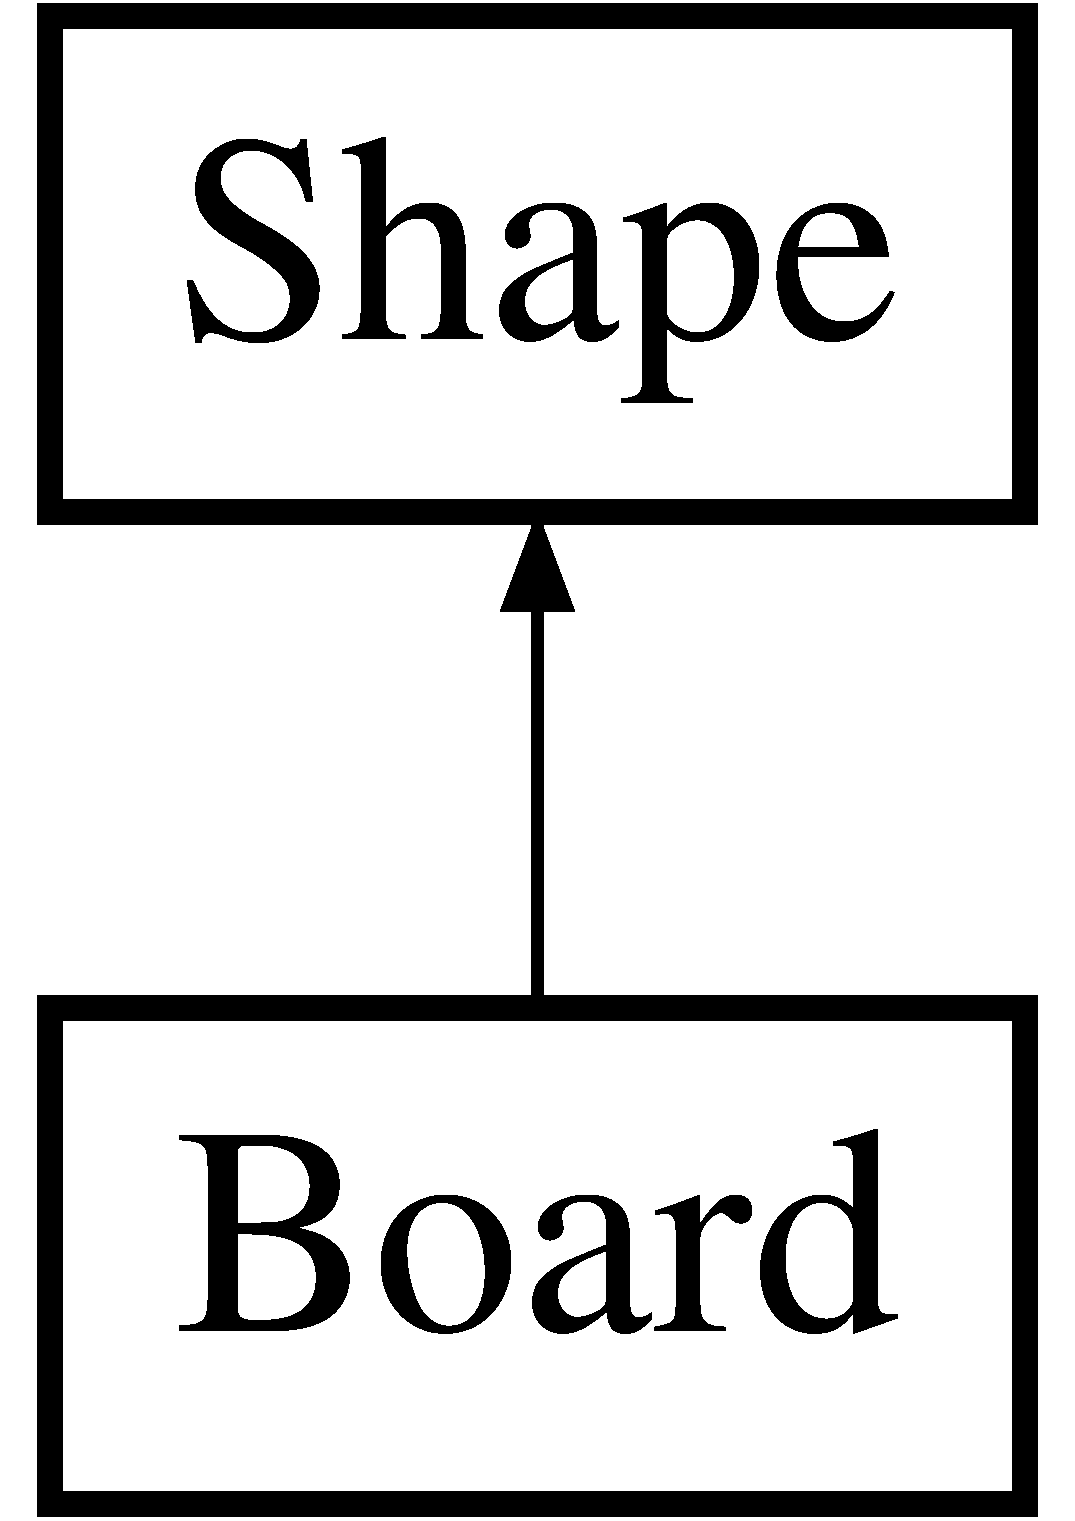
\includegraphics[height=3.000000cm]{class_board}
\end{center}
\end{figure}
\subsection*{Public Member Functions}
\begin{DoxyCompactItemize}
\item 
virtual \mbox{\hyperlink{class_board_af73f45730119a1fd8f6670f53f959e68}{$\sim$\+Board}} ()
\item 
virtual void \mbox{\hyperlink{class_board_afa3fa04776e43db38f3f1dd9bba28e6e}{set\+Color}} (const \mbox{\hyperlink{class_r_g_b_color}{R\+G\+B\+Color}} \&color)
\begin{DoxyCompactList}\small\item\em Set color of the whole board. \end{DoxyCompactList}\item 
virtual void \mbox{\hyperlink{class_board_a9c8fc3e645f56bec246a27459f5c75ec}{set\+Unit\+Square\+Color}} (const int \&i, const int \&j, const \mbox{\hyperlink{class_r_g_b_color}{R\+G\+B\+Color}} \&c)
\item 
virtual \mbox{\hyperlink{class_r_g_b_color}{R\+G\+B\+Color}} \mbox{\hyperlink{class_board_a6e6a947ec66c09bff4559fd9650b9b1d}{get\+Unit\+Square\+Color}} (const int \&i, const int \&j) const
\item 
virtual void \mbox{\hyperlink{class_board_af74f0d4b43e5aa3faea16d7c6407b05e}{clear}} ()
\begin{DoxyCompactList}\small\item\em Clear the board. \end{DoxyCompactList}\item 
virtual bool \mbox{\hyperlink{class_board_a497025aedeebf35030eb7e99972de4e1}{can\+Place\+Shape\+At\+Pos}} (const \mbox{\hyperlink{class_shape}{Shape}} $\ast$piece, const int \&i\+\_\+origin, const int \&j\+\_\+origin) const
\begin{DoxyCompactList}\small\item\em Check whether the chosen piece can be placed at specific position. \end{DoxyCompactList}\item 
virtual bool \mbox{\hyperlink{class_board_a0bf419d10b557cd2119ba7f2fcec7471}{is\+Any\+Space\+Placeable}} (const \mbox{\hyperlink{class_shape}{Shape}} $\ast$piece) const
\begin{DoxyCompactList}\small\item\em Check whether the chosen piece can be placed onto the board. \end{DoxyCompactList}\item 
virtual void \mbox{\hyperlink{class_board_a759fee79a5c0da27101adc909c352b62}{place}} (\mbox{\hyperlink{class_visible_shape}{Visible\+Shape}} $\ast$piece, const int \&i\+\_\+origin, const int \&j\+\_\+origin, \mbox{\hyperlink{class_encrypted_num}{Encrypted\+Num}} $\ast$score)
\begin{DoxyCompactList}\small\item\em Place the piece onto the board and update the score. \end{DoxyCompactList}\item 
virtual std\+::pair$<$ int, int $>$ \mbox{\hyperlink{class_board_a47fb67404ee45b4ad700a57e3849995b}{get\+Unit\+Square\+Pos}} (int mouse\+\_\+x, int mouse\+\_\+y, const \mbox{\hyperlink{class_visible_shape}{Visible\+Shape}} $\ast$piece) const
\begin{DoxyCompactList}\small\item\em Find the top-\/left unit square being overlapped by the piece. \end{DoxyCompactList}\item 
virtual bool \mbox{\hyperlink{class_board_aa4001c8b1e2338fa0dfed7df6f5dcb6b}{can\+Place\+Shape\+At\+Coordinate}} (const \mbox{\hyperlink{class_visible_shape}{Visible\+Shape}} $\ast$piece, const int \&mouse\+\_\+x, const int \&mouse\+\_\+y) const
\begin{DoxyCompactList}\small\item\em Check whether the chosen piece can be placed with mouse at specific coordinate. \end{DoxyCompactList}\item 
virtual void \mbox{\hyperlink{class_board_a6403c0a5182a07188fd0011748f27e9c}{place\+Mouse}} (\mbox{\hyperlink{class_visible_shape}{Visible\+Shape}} $\ast$piece, const int \&mouse\+\_\+x, const int \&mouse\+\_\+y, \mbox{\hyperlink{class_encrypted_num}{Encrypted\+Num}} $\ast$score)
\begin{DoxyCompactList}\small\item\em Place the piece onto the board by mouse and update the score. \end{DoxyCompactList}\item 
virtual \mbox{\hyperlink{class_visible_shape}{Visible\+Shape}} \mbox{\hyperlink{class_board_a51f08756175c14dd36acfcdf3b9ea356}{preview}} (\mbox{\hyperlink{class_visible_shape}{Visible\+Shape}} piece, const int \&mouse\+\_\+x, const int \&mouse\+\_\+y, const std\+::string \&path\+\_\+reverse) const
\begin{DoxyCompactList}\small\item\em Preview the piece before it is placed. \end{DoxyCompactList}\item 
virtual \mbox{\hyperlink{class_board}{Board}} \mbox{\hyperlink{class_board_aeff7b135ffeea47ce26da75ce670807a}{sub}} (const int \&x, const int \&y, const int \&w, const int \&h) const
\begin{DoxyCompactList}\small\item\em Get a part of the board. \end{DoxyCompactList}\item 
\mbox{\hyperlink{class_board_a280deeca2a39d227887ff2e13b009c0a}{Visible\+Shape}} ()
\item 
\mbox{\hyperlink{class_board_adc9d11f72af8b96fdb379330fd9de592}{Visible\+Shape}} (const unsigned int \&row, const unsigned int \&col)
\begin{DoxyCompactList}\small\item\em constructor for filled rectangle \end{DoxyCompactList}\item 
\mbox{\hyperlink{class_board_a0efa89e218acbaeaf4f2453467d54cc9}{Visible\+Shape}} (const std\+::vector$<$ std\+::vector$<$ bool $>$ $>$ \&bitmap)
\begin{DoxyCompactList}\small\item\em constructor for any shape \end{DoxyCompactList}\end{DoxyCompactItemize}


\subsection{Detailed Description}
The board where pieces are placed. 

\mbox{\hyperlink{class_board}{Board}} is a derived class from \mbox{\hyperlink{class_visible_shape}{Visible\+Shape}}. 

\subsection{Constructor \& Destructor Documentation}
\mbox{\Hypertarget{class_board_af73f45730119a1fd8f6670f53f959e68}\label{class_board_af73f45730119a1fd8f6670f53f959e68}} 
\index{Board@{Board}!````~Board@{$\sim$\+Board}}
\index{````~Board@{$\sim$\+Board}!Board@{Board}}
\subsubsection{\texorpdfstring{$\sim$\+Board()}{~Board()}}
{\footnotesize\ttfamily Board\+::$\sim$\+Board (\begin{DoxyParamCaption}{ }\end{DoxyParamCaption})\hspace{0.3cm}{\ttfamily [virtual]}}



\subsection{Member Function Documentation}
\mbox{\Hypertarget{class_board_aa4001c8b1e2338fa0dfed7df6f5dcb6b}\label{class_board_aa4001c8b1e2338fa0dfed7df6f5dcb6b}} 
\index{Board@{Board}!can\+Place\+Shape\+At\+Coordinate@{can\+Place\+Shape\+At\+Coordinate}}
\index{can\+Place\+Shape\+At\+Coordinate@{can\+Place\+Shape\+At\+Coordinate}!Board@{Board}}
\subsubsection{\texorpdfstring{can\+Place\+Shape\+At\+Coordinate()}{canPlaceShapeAtCoordinate()}}
{\footnotesize\ttfamily bool Board\+::can\+Place\+Shape\+At\+Coordinate (\begin{DoxyParamCaption}\item[{const \mbox{\hyperlink{class_visible_shape}{Visible\+Shape}} $\ast$}]{piece,  }\item[{const int \&}]{mouse\+\_\+x,  }\item[{const int \&}]{mouse\+\_\+y }\end{DoxyParamCaption}) const\hspace{0.3cm}{\ttfamily [virtual]}}



Check whether the chosen piece can be placed with mouse at specific coordinate. 


\begin{DoxyParams}{Parameters}
{\em mouse\+\_\+x} & The x coordinate of the mouse \\
\hline
{\em mouse\+\_\+y} & The y coordinate of the mouse \\
\hline
{\em piece} & The chosen piece \\
\hline
\end{DoxyParams}
\mbox{\Hypertarget{class_board_a497025aedeebf35030eb7e99972de4e1}\label{class_board_a497025aedeebf35030eb7e99972de4e1}} 
\index{Board@{Board}!can\+Place\+Shape\+At\+Pos@{can\+Place\+Shape\+At\+Pos}}
\index{can\+Place\+Shape\+At\+Pos@{can\+Place\+Shape\+At\+Pos}!Board@{Board}}
\subsubsection{\texorpdfstring{can\+Place\+Shape\+At\+Pos()}{canPlaceShapeAtPos()}}
{\footnotesize\ttfamily bool Board\+::can\+Place\+Shape\+At\+Pos (\begin{DoxyParamCaption}\item[{const \mbox{\hyperlink{class_shape}{Shape}} $\ast$}]{piece,  }\item[{const int \&}]{i\+\_\+origin,  }\item[{const int \&}]{j\+\_\+origin }\end{DoxyParamCaption}) const\hspace{0.3cm}{\ttfamily [virtual]}}



Check whether the chosen piece can be placed at specific position. 


\begin{DoxyParams}{Parameters}
{\em piece} & The chosen piece \\
\hline
{\em i\+\_\+origin} & The topmost row being placed onto \\
\hline
{\em j\+\_\+origin} & The leftmost column begin placed onto \\
\hline
\end{DoxyParams}
\mbox{\Hypertarget{class_board_af74f0d4b43e5aa3faea16d7c6407b05e}\label{class_board_af74f0d4b43e5aa3faea16d7c6407b05e}} 
\index{Board@{Board}!clear@{clear}}
\index{clear@{clear}!Board@{Board}}
\subsubsection{\texorpdfstring{clear()}{clear()}}
{\footnotesize\ttfamily void Board\+::clear (\begin{DoxyParamCaption}{ }\end{DoxyParamCaption})\hspace{0.3cm}{\ttfamily [virtual]}}



Clear the board. 

\mbox{\Hypertarget{class_board_a6e6a947ec66c09bff4559fd9650b9b1d}\label{class_board_a6e6a947ec66c09bff4559fd9650b9b1d}} 
\index{Board@{Board}!get\+Unit\+Square\+Color@{get\+Unit\+Square\+Color}}
\index{get\+Unit\+Square\+Color@{get\+Unit\+Square\+Color}!Board@{Board}}
\subsubsection{\texorpdfstring{get\+Unit\+Square\+Color()}{getUnitSquareColor()}}
{\footnotesize\ttfamily \mbox{\hyperlink{class_r_g_b_color}{R\+G\+B\+Color}} Board\+::get\+Unit\+Square\+Color (\begin{DoxyParamCaption}\item[{const int \&}]{i,  }\item[{const int \&}]{j }\end{DoxyParamCaption}) const\hspace{0.3cm}{\ttfamily [virtual]}}

\begin{DoxySeeAlso}{See also}
\mbox{\hyperlink{class_board_a9c8fc3e645f56bec246a27459f5c75ec}{set\+Unit\+Square\+Color()}} 
\end{DoxySeeAlso}
\mbox{\Hypertarget{class_board_a47fb67404ee45b4ad700a57e3849995b}\label{class_board_a47fb67404ee45b4ad700a57e3849995b}} 
\index{Board@{Board}!get\+Unit\+Square\+Pos@{get\+Unit\+Square\+Pos}}
\index{get\+Unit\+Square\+Pos@{get\+Unit\+Square\+Pos}!Board@{Board}}
\subsubsection{\texorpdfstring{get\+Unit\+Square\+Pos()}{getUnitSquarePos()}}
{\footnotesize\ttfamily std\+::pair$<$ int, int $>$ Board\+::get\+Unit\+Square\+Pos (\begin{DoxyParamCaption}\item[{int}]{mouse\+\_\+x,  }\item[{int}]{mouse\+\_\+y,  }\item[{const \mbox{\hyperlink{class_visible_shape}{Visible\+Shape}} $\ast$}]{piece }\end{DoxyParamCaption}) const\hspace{0.3cm}{\ttfamily [virtual]}}



Find the top-\/left unit square being overlapped by the piece. 


\begin{DoxyParams}{Parameters}
{\em mouse\+\_\+x} & The x coordinate of the mouse \\
\hline
{\em mouse\+\_\+y} & The y coordinate of the mouse \\
\hline
{\em piece} & The chosen piece \\
\hline
\end{DoxyParams}
\begin{DoxyReturn}{Returns}
The position of the unit square 
\end{DoxyReturn}
\mbox{\Hypertarget{class_board_a0bf419d10b557cd2119ba7f2fcec7471}\label{class_board_a0bf419d10b557cd2119ba7f2fcec7471}} 
\index{Board@{Board}!is\+Any\+Space\+Placeable@{is\+Any\+Space\+Placeable}}
\index{is\+Any\+Space\+Placeable@{is\+Any\+Space\+Placeable}!Board@{Board}}
\subsubsection{\texorpdfstring{is\+Any\+Space\+Placeable()}{isAnySpacePlaceable()}}
{\footnotesize\ttfamily bool Board\+::is\+Any\+Space\+Placeable (\begin{DoxyParamCaption}\item[{const \mbox{\hyperlink{class_shape}{Shape}} $\ast$}]{piece }\end{DoxyParamCaption}) const\hspace{0.3cm}{\ttfamily [virtual]}}



Check whether the chosen piece can be placed onto the board. 


\begin{DoxyParams}{Parameters}
{\em piece} & The chosen piece \\
\hline
\end{DoxyParams}
\mbox{\Hypertarget{class_board_a759fee79a5c0da27101adc909c352b62}\label{class_board_a759fee79a5c0da27101adc909c352b62}} 
\index{Board@{Board}!place@{place}}
\index{place@{place}!Board@{Board}}
\subsubsection{\texorpdfstring{place()}{place()}}
{\footnotesize\ttfamily void Board\+::place (\begin{DoxyParamCaption}\item[{\mbox{\hyperlink{class_visible_shape}{Visible\+Shape}} $\ast$}]{piece,  }\item[{const int \&}]{i\+\_\+origin,  }\item[{const int \&}]{j\+\_\+origin,  }\item[{\mbox{\hyperlink{class_encrypted_num}{Encrypted\+Num}} $\ast$}]{score }\end{DoxyParamCaption})\hspace{0.3cm}{\ttfamily [virtual]}}



Place the piece onto the board and update the score. 


\begin{DoxyParams}{Parameters}
{\em piece} & The chosen piece \\
\hline
{\em i\+\_\+origin} & The topmost row being placed onto \\
\hline
{\em j\+\_\+origin} & The leftmost column begin placed onto \\
\hline
{\em score} & Score being updated \\
\hline
\end{DoxyParams}
Clear lines when they are completed \mbox{\Hypertarget{class_board_a6403c0a5182a07188fd0011748f27e9c}\label{class_board_a6403c0a5182a07188fd0011748f27e9c}} 
\index{Board@{Board}!place\+Mouse@{place\+Mouse}}
\index{place\+Mouse@{place\+Mouse}!Board@{Board}}
\subsubsection{\texorpdfstring{place\+Mouse()}{placeMouse()}}
{\footnotesize\ttfamily void Board\+::place\+Mouse (\begin{DoxyParamCaption}\item[{\mbox{\hyperlink{class_visible_shape}{Visible\+Shape}} $\ast$}]{piece,  }\item[{const int \&}]{mouse\+\_\+x,  }\item[{const int \&}]{mouse\+\_\+y,  }\item[{\mbox{\hyperlink{class_encrypted_num}{Encrypted\+Num}} $\ast$}]{score }\end{DoxyParamCaption})\hspace{0.3cm}{\ttfamily [virtual]}}



Place the piece onto the board by mouse and update the score. 


\begin{DoxyParams}{Parameters}
{\em piece} & The chosen piece \\
\hline
{\em mouse\+\_\+x} & The x coordinate of the mouse \\
\hline
{\em mouse\+\_\+y} & The y coordinate of the mouse \\
\hline
{\em score} & Score being updated \\
\hline
\end{DoxyParams}
\mbox{\Hypertarget{class_board_a51f08756175c14dd36acfcdf3b9ea356}\label{class_board_a51f08756175c14dd36acfcdf3b9ea356}} 
\index{Board@{Board}!preview@{preview}}
\index{preview@{preview}!Board@{Board}}
\subsubsection{\texorpdfstring{preview()}{preview()}}
{\footnotesize\ttfamily \mbox{\hyperlink{class_visible_shape}{Visible\+Shape}} Board\+::preview (\begin{DoxyParamCaption}\item[{\mbox{\hyperlink{class_visible_shape}{Visible\+Shape}}}]{piece,  }\item[{const int \&}]{mouse\+\_\+x,  }\item[{const int \&}]{mouse\+\_\+y,  }\item[{const std\+::string \&}]{path\+\_\+reverse }\end{DoxyParamCaption}) const\hspace{0.3cm}{\ttfamily [virtual]}}



Preview the piece before it is placed. 


\begin{DoxyParams}{Parameters}
{\em piece} & The chosen piece \\
\hline
{\em mouse\+\_\+x} & The x coordinate of the mouse \\
\hline
{\em mouse\+\_\+y} & The y coordinate of the mouse \\
\hline
{\em path\+\_\+reverse} & The path pointing to the border image \\
\hline
\end{DoxyParams}
\begin{DoxyReturn}{Returns}
A pointer to the piece with a view to rendering it 
\end{DoxyReturn}
\mbox{\Hypertarget{class_board_afa3fa04776e43db38f3f1dd9bba28e6e}\label{class_board_afa3fa04776e43db38f3f1dd9bba28e6e}} 
\index{Board@{Board}!set\+Color@{set\+Color}}
\index{set\+Color@{set\+Color}!Board@{Board}}
\subsubsection{\texorpdfstring{set\+Color()}{setColor()}}
{\footnotesize\ttfamily void Board\+::set\+Color (\begin{DoxyParamCaption}\item[{const \mbox{\hyperlink{class_r_g_b_color}{R\+G\+B\+Color}} \&}]{color }\end{DoxyParamCaption})\hspace{0.3cm}{\ttfamily [virtual]}}



Set color of the whole board. 

\begin{DoxySeeAlso}{See also}
Shape\+::set\+Color() 
\end{DoxySeeAlso}


Reimplemented from \mbox{\hyperlink{class_visible_shape_a69ae0940d090fec376bee8dc6861b8dc}{Visible\+Shape}}.

\mbox{\Hypertarget{class_board_a9c8fc3e645f56bec246a27459f5c75ec}\label{class_board_a9c8fc3e645f56bec246a27459f5c75ec}} 
\index{Board@{Board}!set\+Unit\+Square\+Color@{set\+Unit\+Square\+Color}}
\index{set\+Unit\+Square\+Color@{set\+Unit\+Square\+Color}!Board@{Board}}
\subsubsection{\texorpdfstring{set\+Unit\+Square\+Color()}{setUnitSquareColor()}}
{\footnotesize\ttfamily void Board\+::set\+Unit\+Square\+Color (\begin{DoxyParamCaption}\item[{const int \&}]{i,  }\item[{const int \&}]{j,  }\item[{const \mbox{\hyperlink{class_r_g_b_color}{R\+G\+B\+Color}} \&}]{c }\end{DoxyParamCaption})\hspace{0.3cm}{\ttfamily [virtual]}}

\begin{DoxySeeAlso}{See also}
\mbox{\hyperlink{class_board_a6e6a947ec66c09bff4559fd9650b9b1d}{get\+Unit\+Square\+Color()}} 
\end{DoxySeeAlso}
\mbox{\Hypertarget{class_board_aeff7b135ffeea47ce26da75ce670807a}\label{class_board_aeff7b135ffeea47ce26da75ce670807a}} 
\index{Board@{Board}!sub@{sub}}
\index{sub@{sub}!Board@{Board}}
\subsubsection{\texorpdfstring{sub()}{sub()}}
{\footnotesize\ttfamily \mbox{\hyperlink{class_board}{Board}} Board\+::sub (\begin{DoxyParamCaption}\item[{const int \&}]{x,  }\item[{const int \&}]{y,  }\item[{const int \&}]{w,  }\item[{const int \&}]{h }\end{DoxyParamCaption}) const\hspace{0.3cm}{\ttfamily [virtual]}}



Get a part of the board. 

\mbox{\Hypertarget{class_board_a280deeca2a39d227887ff2e13b009c0a}\label{class_board_a280deeca2a39d227887ff2e13b009c0a}} 
\index{Board@{Board}!Visible\+Shape@{Visible\+Shape}}
\index{Visible\+Shape@{Visible\+Shape}!Board@{Board}}
\subsubsection{\texorpdfstring{Visible\+Shape()}{VisibleShape()}\hspace{0.1cm}{\footnotesize\ttfamily [1/3]}}
{\footnotesize\ttfamily Visible\+Shape\+::\+Visible\+Shape}

\mbox{\Hypertarget{class_board_a0efa89e218acbaeaf4f2453467d54cc9}\label{class_board_a0efa89e218acbaeaf4f2453467d54cc9}} 
\index{Board@{Board}!Visible\+Shape@{Visible\+Shape}}
\index{Visible\+Shape@{Visible\+Shape}!Board@{Board}}
\subsubsection{\texorpdfstring{Visible\+Shape()}{VisibleShape()}\hspace{0.1cm}{\footnotesize\ttfamily [2/3]}}
{\footnotesize\ttfamily Visible\+Shape\+::\+Visible\+Shape}



constructor for any shape 


\begin{DoxyParams}{Parameters}
{\em bitmap} & The bitmap representing the shape. \\
\hline
\end{DoxyParams}
\begin{DoxySeeAlso}{See also}
\mbox{\hyperlink{class_shape_ae79ee483d0f48a426d1a544fd22fd8e5}{set\+Bit\+Map()}} 
\end{DoxySeeAlso}
\mbox{\Hypertarget{class_board_adc9d11f72af8b96fdb379330fd9de592}\label{class_board_adc9d11f72af8b96fdb379330fd9de592}} 
\index{Board@{Board}!Visible\+Shape@{Visible\+Shape}}
\index{Visible\+Shape@{Visible\+Shape}!Board@{Board}}
\subsubsection{\texorpdfstring{Visible\+Shape()}{VisibleShape()}\hspace{0.1cm}{\footnotesize\ttfamily [3/3]}}
{\footnotesize\ttfamily Visible\+Shape\+::\+Visible\+Shape}



constructor for filled rectangle 


\begin{DoxyParams}{Parameters}
{\em row} & The number of rows of the rectangle \\
\hline
{\em col} & The number of columns of the rectangle \\
\hline
\end{DoxyParams}


The documentation for this class was generated from the following files\+:\begin{DoxyCompactItemize}
\item 
\mbox{\hyperlink{board_8h}{board.\+h}}\item 
\mbox{\hyperlink{board_8cpp}{board.\+cpp}}\end{DoxyCompactItemize}

\hypertarget{class_button}{}\section{Button Class Reference}
\label{class_button}\index{Button@{Button}}


A class that defines button including icon and text.  




{\ttfamily \#include $<$button.\+h$>$}

\subsection*{Public Member Functions}
\begin{DoxyCompactItemize}
\item 
\mbox{\hyperlink{class_button_a3b36df1ae23c58aedb9e15a713159459}{Button}} ()
\item 
\mbox{\hyperlink{class_button_a0afd720661614d65ec8f59a20ba2e1d0}{Button}} (const \mbox{\hyperlink{class_image}{Image}} \&icon, \mbox{\hyperlink{class_font}{Font}} title=\mbox{\hyperlink{class_font}{Font}}(\char`\"{}\char`\"{}, \char`\"{}\char`\"{}))
\item 
\mbox{\hyperlink{class_button_aeec07db7dcdbf546a152b2056c167a4a}{Button}} (const \mbox{\hyperlink{class_font}{Font}} \&title)
\item 
virtual \mbox{\hyperlink{class_button_a2a001eb9c3cc8ae54768a850dd345002}{$\sim$\+Button}} ()
\item 
virtual void \mbox{\hyperlink{class_button_aabe6ae612c78c4e49d6c4de222e3dcb2}{set\+Icon}} (const \mbox{\hyperlink{class_image}{Image}} \&icon)
\item 
virtual \mbox{\hyperlink{class_image}{Image}} \mbox{\hyperlink{class_button_afc946623026b3f18de86af8e4cc2921e}{get\+Icon}} () const
\item 
virtual void \mbox{\hyperlink{class_button_aca4632ad68e021d147966c8782917f83}{set\+Title}} (const \mbox{\hyperlink{class_font}{Font}} \&title)
\item 
virtual \mbox{\hyperlink{class_font}{Font}} \mbox{\hyperlink{class_button_afd5d30f0dc6aba866c45072c59ee06f8}{get\+Title}} () const
\item 
virtual void \mbox{\hyperlink{class_button_a87418f0a2d9ecbff822627e4e728728e}{set\+Color}} (const \mbox{\hyperlink{class_r_g_b_color}{R\+G\+B\+Color}} \&color)
\begin{DoxyCompactList}\small\item\em Set the color of the title. \end{DoxyCompactList}\item 
virtual \mbox{\hyperlink{class_r_g_b_color}{R\+G\+B\+Color}} \mbox{\hyperlink{class_button_a3388931e8e8cef41336f973578304c8a}{get\+Color}} () const
\begin{DoxyCompactList}\small\item\em Get the color of the title. \end{DoxyCompactList}\item 
virtual void \mbox{\hyperlink{class_button_a808e7d56490172fdeab84afb01fc4bde}{set\+Coordinate}} (const int \&x, const int \&y)
\begin{DoxyCompactList}\small\item\em Set the coordinate of the top-\/left corner of the button. \end{DoxyCompactList}\item 
virtual int \mbox{\hyperlink{class_button_a05c6aae1cf037ad66e3821963fe72988}{getX}} () const
\begin{DoxyCompactList}\small\item\em Get the x coordinate of the button. \end{DoxyCompactList}\item 
virtual int \mbox{\hyperlink{class_button_a3acf216100c43b999e38047bfdf99ee7}{getY}} () const
\begin{DoxyCompactList}\small\item\em Get the y coordinate of the button. \end{DoxyCompactList}\item 
virtual void \mbox{\hyperlink{class_button_a6b048681f073eae03631251ddee96b17}{set\+Height}} (const unsigned int \&height)
\item 
virtual int \mbox{\hyperlink{class_button_ab4e3a35e683df269eb4b178632694dbf}{get\+Height}} () const
\item 
virtual void \mbox{\hyperlink{class_button_a77d90f51ba19a275e9d662cbb081049f}{set\+Width}} (const unsigned int \&width)
\item 
virtual int \mbox{\hyperlink{class_button_a75acf94e1d23db5a64830c8ea7280c0a}{get\+Width}} () const
\item 
virtual bool \mbox{\hyperlink{class_button_ac2449ee251bb58bb505b3b6c825d4129}{inside}} (const int \&x, const int \&y)
\begin{DoxyCompactList}\small\item\em Check whether the mouse currently points at the button. \end{DoxyCompactList}\end{DoxyCompactItemize}


\subsection{Detailed Description}
A class that defines button including icon and text. 

\subsection{Constructor \& Destructor Documentation}
\mbox{\Hypertarget{class_button_a3b36df1ae23c58aedb9e15a713159459}\label{class_button_a3b36df1ae23c58aedb9e15a713159459}} 
\index{Button@{Button}!Button@{Button}}
\index{Button@{Button}!Button@{Button}}
\subsubsection{\texorpdfstring{Button()}{Button()}\hspace{0.1cm}{\footnotesize\ttfamily [1/3]}}
{\footnotesize\ttfamily Button\+::\+Button (\begin{DoxyParamCaption}{ }\end{DoxyParamCaption})}

\mbox{\Hypertarget{class_button_a0afd720661614d65ec8f59a20ba2e1d0}\label{class_button_a0afd720661614d65ec8f59a20ba2e1d0}} 
\index{Button@{Button}!Button@{Button}}
\index{Button@{Button}!Button@{Button}}
\subsubsection{\texorpdfstring{Button()}{Button()}\hspace{0.1cm}{\footnotesize\ttfamily [2/3]}}
{\footnotesize\ttfamily Button\+::\+Button (\begin{DoxyParamCaption}\item[{const \mbox{\hyperlink{class_image}{Image}} \&}]{icon,  }\item[{\mbox{\hyperlink{class_font}{Font}}}]{title = {\ttfamily \mbox{\hyperlink{class_font}{Font}}(\char`\"{}\char`\"{},~\char`\"{}\char`\"{})} }\end{DoxyParamCaption})}

\mbox{\Hypertarget{class_button_aeec07db7dcdbf546a152b2056c167a4a}\label{class_button_aeec07db7dcdbf546a152b2056c167a4a}} 
\index{Button@{Button}!Button@{Button}}
\index{Button@{Button}!Button@{Button}}
\subsubsection{\texorpdfstring{Button()}{Button()}\hspace{0.1cm}{\footnotesize\ttfamily [3/3]}}
{\footnotesize\ttfamily Button\+::\+Button (\begin{DoxyParamCaption}\item[{const \mbox{\hyperlink{class_font}{Font}} \&}]{title }\end{DoxyParamCaption})}

\mbox{\Hypertarget{class_button_a2a001eb9c3cc8ae54768a850dd345002}\label{class_button_a2a001eb9c3cc8ae54768a850dd345002}} 
\index{Button@{Button}!````~Button@{$\sim$\+Button}}
\index{````~Button@{$\sim$\+Button}!Button@{Button}}
\subsubsection{\texorpdfstring{$\sim$\+Button()}{~Button()}}
{\footnotesize\ttfamily Button\+::$\sim$\+Button (\begin{DoxyParamCaption}{ }\end{DoxyParamCaption})\hspace{0.3cm}{\ttfamily [virtual]}}



\subsection{Member Function Documentation}
\mbox{\Hypertarget{class_button_a3388931e8e8cef41336f973578304c8a}\label{class_button_a3388931e8e8cef41336f973578304c8a}} 
\index{Button@{Button}!get\+Color@{get\+Color}}
\index{get\+Color@{get\+Color}!Button@{Button}}
\subsubsection{\texorpdfstring{get\+Color()}{getColor()}}
{\footnotesize\ttfamily \mbox{\hyperlink{class_r_g_b_color}{R\+G\+B\+Color}} Button\+::get\+Color (\begin{DoxyParamCaption}{ }\end{DoxyParamCaption}) const\hspace{0.3cm}{\ttfamily [virtual]}}



Get the color of the title. 

\begin{DoxySeeAlso}{See also}
\mbox{\hyperlink{class_button_a87418f0a2d9ecbff822627e4e728728e}{set\+Color()}} 
\end{DoxySeeAlso}
\mbox{\Hypertarget{class_button_ab4e3a35e683df269eb4b178632694dbf}\label{class_button_ab4e3a35e683df269eb4b178632694dbf}} 
\index{Button@{Button}!get\+Height@{get\+Height}}
\index{get\+Height@{get\+Height}!Button@{Button}}
\subsubsection{\texorpdfstring{get\+Height()}{getHeight()}}
{\footnotesize\ttfamily int Button\+::get\+Height (\begin{DoxyParamCaption}{ }\end{DoxyParamCaption}) const\hspace{0.3cm}{\ttfamily [virtual]}}

\begin{DoxySeeAlso}{See also}
\mbox{\hyperlink{class_button_a6b048681f073eae03631251ddee96b17}{set\+Height()}} 
\end{DoxySeeAlso}
\mbox{\Hypertarget{class_button_afc946623026b3f18de86af8e4cc2921e}\label{class_button_afc946623026b3f18de86af8e4cc2921e}} 
\index{Button@{Button}!get\+Icon@{get\+Icon}}
\index{get\+Icon@{get\+Icon}!Button@{Button}}
\subsubsection{\texorpdfstring{get\+Icon()}{getIcon()}}
{\footnotesize\ttfamily \mbox{\hyperlink{class_image}{Image}} Button\+::get\+Icon (\begin{DoxyParamCaption}{ }\end{DoxyParamCaption}) const\hspace{0.3cm}{\ttfamily [virtual]}}

\begin{DoxySeeAlso}{See also}
\mbox{\hyperlink{class_button_aabe6ae612c78c4e49d6c4de222e3dcb2}{set\+Icon()}} 
\end{DoxySeeAlso}
\mbox{\Hypertarget{class_button_afd5d30f0dc6aba866c45072c59ee06f8}\label{class_button_afd5d30f0dc6aba866c45072c59ee06f8}} 
\index{Button@{Button}!get\+Title@{get\+Title}}
\index{get\+Title@{get\+Title}!Button@{Button}}
\subsubsection{\texorpdfstring{get\+Title()}{getTitle()}}
{\footnotesize\ttfamily \mbox{\hyperlink{class_font}{Font}} Button\+::get\+Title (\begin{DoxyParamCaption}{ }\end{DoxyParamCaption}) const\hspace{0.3cm}{\ttfamily [virtual]}}

\begin{DoxySeeAlso}{See also}
\mbox{\hyperlink{class_button_aca4632ad68e021d147966c8782917f83}{set\+Title()}} 
\end{DoxySeeAlso}
\mbox{\Hypertarget{class_button_a75acf94e1d23db5a64830c8ea7280c0a}\label{class_button_a75acf94e1d23db5a64830c8ea7280c0a}} 
\index{Button@{Button}!get\+Width@{get\+Width}}
\index{get\+Width@{get\+Width}!Button@{Button}}
\subsubsection{\texorpdfstring{get\+Width()}{getWidth()}}
{\footnotesize\ttfamily int Button\+::get\+Width (\begin{DoxyParamCaption}{ }\end{DoxyParamCaption}) const\hspace{0.3cm}{\ttfamily [virtual]}}

\begin{DoxySeeAlso}{See also}
\mbox{\hyperlink{class_button_a77d90f51ba19a275e9d662cbb081049f}{set\+Width()}} 
\end{DoxySeeAlso}
\mbox{\Hypertarget{class_button_a05c6aae1cf037ad66e3821963fe72988}\label{class_button_a05c6aae1cf037ad66e3821963fe72988}} 
\index{Button@{Button}!getX@{getX}}
\index{getX@{getX}!Button@{Button}}
\subsubsection{\texorpdfstring{get\+X()}{getX()}}
{\footnotesize\ttfamily int Button\+::getX (\begin{DoxyParamCaption}{ }\end{DoxyParamCaption}) const\hspace{0.3cm}{\ttfamily [virtual]}}



Get the x coordinate of the button. 

\begin{DoxySeeAlso}{See also}
\mbox{\hyperlink{class_button_a808e7d56490172fdeab84afb01fc4bde}{set\+Coordinate()}}; 
\end{DoxySeeAlso}
\mbox{\Hypertarget{class_button_a3acf216100c43b999e38047bfdf99ee7}\label{class_button_a3acf216100c43b999e38047bfdf99ee7}} 
\index{Button@{Button}!getY@{getY}}
\index{getY@{getY}!Button@{Button}}
\subsubsection{\texorpdfstring{get\+Y()}{getY()}}
{\footnotesize\ttfamily int Button\+::getY (\begin{DoxyParamCaption}{ }\end{DoxyParamCaption}) const\hspace{0.3cm}{\ttfamily [virtual]}}



Get the y coordinate of the button. 

\begin{DoxySeeAlso}{See also}
\mbox{\hyperlink{class_button_a808e7d56490172fdeab84afb01fc4bde}{set\+Coordinate()}}; 
\end{DoxySeeAlso}
\mbox{\Hypertarget{class_button_ac2449ee251bb58bb505b3b6c825d4129}\label{class_button_ac2449ee251bb58bb505b3b6c825d4129}} 
\index{Button@{Button}!inside@{inside}}
\index{inside@{inside}!Button@{Button}}
\subsubsection{\texorpdfstring{inside()}{inside()}}
{\footnotesize\ttfamily bool Button\+::inside (\begin{DoxyParamCaption}\item[{const int \&}]{x,  }\item[{const int \&}]{y }\end{DoxyParamCaption})\hspace{0.3cm}{\ttfamily [virtual]}}



Check whether the mouse currently points at the button. 

Always return false if the size of the button has never been set before 
\begin{DoxyParams}{Parameters}
{\em x} & The x coordinate of the mouse \\
\hline
{\em y} & The y coordinate of the mouse \\
\hline
\end{DoxyParams}
\begin{DoxySeeAlso}{See also}
\mbox{\hyperlink{class_button_a6b048681f073eae03631251ddee96b17}{set\+Height()}} 

\mbox{\hyperlink{class_button_a77d90f51ba19a275e9d662cbb081049f}{set\+Width()}} 
\end{DoxySeeAlso}
\mbox{\Hypertarget{class_button_a87418f0a2d9ecbff822627e4e728728e}\label{class_button_a87418f0a2d9ecbff822627e4e728728e}} 
\index{Button@{Button}!set\+Color@{set\+Color}}
\index{set\+Color@{set\+Color}!Button@{Button}}
\subsubsection{\texorpdfstring{set\+Color()}{setColor()}}
{\footnotesize\ttfamily void Button\+::set\+Color (\begin{DoxyParamCaption}\item[{const \mbox{\hyperlink{class_r_g_b_color}{R\+G\+B\+Color}} \&}]{color }\end{DoxyParamCaption})\hspace{0.3cm}{\ttfamily [virtual]}}



Set the color of the title. 

\begin{DoxySeeAlso}{See also}
\mbox{\hyperlink{class_button_a3388931e8e8cef41336f973578304c8a}{get\+Color()}} 
\end{DoxySeeAlso}
\mbox{\Hypertarget{class_button_a808e7d56490172fdeab84afb01fc4bde}\label{class_button_a808e7d56490172fdeab84afb01fc4bde}} 
\index{Button@{Button}!set\+Coordinate@{set\+Coordinate}}
\index{set\+Coordinate@{set\+Coordinate}!Button@{Button}}
\subsubsection{\texorpdfstring{set\+Coordinate()}{setCoordinate()}}
{\footnotesize\ttfamily void Button\+::set\+Coordinate (\begin{DoxyParamCaption}\item[{const int \&}]{x,  }\item[{const int \&}]{y }\end{DoxyParamCaption})\hspace{0.3cm}{\ttfamily [virtual]}}



Set the coordinate of the top-\/left corner of the button. 

\begin{DoxySeeAlso}{See also}
\mbox{\hyperlink{class_button_a05c6aae1cf037ad66e3821963fe72988}{get\+X()}} 

\mbox{\hyperlink{class_button_a3acf216100c43b999e38047bfdf99ee7}{get\+Y()}} 
\end{DoxySeeAlso}
\mbox{\Hypertarget{class_button_a6b048681f073eae03631251ddee96b17}\label{class_button_a6b048681f073eae03631251ddee96b17}} 
\index{Button@{Button}!set\+Height@{set\+Height}}
\index{set\+Height@{set\+Height}!Button@{Button}}
\subsubsection{\texorpdfstring{set\+Height()}{setHeight()}}
{\footnotesize\ttfamily void Button\+::set\+Height (\begin{DoxyParamCaption}\item[{const unsigned int \&}]{height }\end{DoxyParamCaption})\hspace{0.3cm}{\ttfamily [virtual]}}

\begin{DoxySeeAlso}{See also}
\mbox{\hyperlink{class_button_ab4e3a35e683df269eb4b178632694dbf}{get\+Height()}} 

\mbox{\hyperlink{class_button_a77d90f51ba19a275e9d662cbb081049f}{set\+Width()}} 
\end{DoxySeeAlso}
\mbox{\Hypertarget{class_button_aabe6ae612c78c4e49d6c4de222e3dcb2}\label{class_button_aabe6ae612c78c4e49d6c4de222e3dcb2}} 
\index{Button@{Button}!set\+Icon@{set\+Icon}}
\index{set\+Icon@{set\+Icon}!Button@{Button}}
\subsubsection{\texorpdfstring{set\+Icon()}{setIcon()}}
{\footnotesize\ttfamily void Button\+::set\+Icon (\begin{DoxyParamCaption}\item[{const \mbox{\hyperlink{class_image}{Image}} \&}]{icon }\end{DoxyParamCaption})\hspace{0.3cm}{\ttfamily [virtual]}}

\begin{DoxySeeAlso}{See also}
\mbox{\hyperlink{class_button_afc946623026b3f18de86af8e4cc2921e}{get\+Icon()}} 
\end{DoxySeeAlso}
\mbox{\Hypertarget{class_button_aca4632ad68e021d147966c8782917f83}\label{class_button_aca4632ad68e021d147966c8782917f83}} 
\index{Button@{Button}!set\+Title@{set\+Title}}
\index{set\+Title@{set\+Title}!Button@{Button}}
\subsubsection{\texorpdfstring{set\+Title()}{setTitle()}}
{\footnotesize\ttfamily void Button\+::set\+Title (\begin{DoxyParamCaption}\item[{const \mbox{\hyperlink{class_font}{Font}} \&}]{title }\end{DoxyParamCaption})\hspace{0.3cm}{\ttfamily [virtual]}}

\begin{DoxySeeAlso}{See also}
\mbox{\hyperlink{class_button_afd5d30f0dc6aba866c45072c59ee06f8}{get\+Title()}} 
\end{DoxySeeAlso}
\mbox{\Hypertarget{class_button_a77d90f51ba19a275e9d662cbb081049f}\label{class_button_a77d90f51ba19a275e9d662cbb081049f}} 
\index{Button@{Button}!set\+Width@{set\+Width}}
\index{set\+Width@{set\+Width}!Button@{Button}}
\subsubsection{\texorpdfstring{set\+Width()}{setWidth()}}
{\footnotesize\ttfamily void Button\+::set\+Width (\begin{DoxyParamCaption}\item[{const unsigned int \&}]{width }\end{DoxyParamCaption})\hspace{0.3cm}{\ttfamily [virtual]}}

\begin{DoxySeeAlso}{See also}
\mbox{\hyperlink{class_button_a75acf94e1d23db5a64830c8ea7280c0a}{get\+Width()}} 

\mbox{\hyperlink{class_button_a6b048681f073eae03631251ddee96b17}{set\+Height()}} 
\end{DoxySeeAlso}


The documentation for this class was generated from the following files\+:\begin{DoxyCompactItemize}
\item 
\mbox{\hyperlink{button_8h}{button.\+h}}\item 
\mbox{\hyperlink{button_8cpp}{button.\+cpp}}\end{DoxyCompactItemize}

\hypertarget{class_color}{}\section{Color Class Reference}
\label{class_color}\index{Color@{Color}}


A class that defines color.  




{\ttfamily \#include $<$color.\+h$>$}

\subsection*{Public Member Functions}
\begin{DoxyCompactItemize}
\item 
\mbox{\hyperlink{class_color_a9a742cbe9f9f4037f5d9f4e81a9b2428}{Color}} ()
\item 
\mbox{\hyperlink{class_color_ae9ef762fa628be655fef146879922545}{Color}} (const Uint8 \&\+\_\+r, const Uint8 \&\+\_\+g, const Uint8 \&\+\_\+b)
\item 
Uint8 \mbox{\hyperlink{class_color_aecb6487557d6eb8386d1a11c37b026fb}{getR}} () const
\begin{DoxyCompactList}\small\item\em get the Red value of the color \end{DoxyCompactList}\item 
Uint8 \mbox{\hyperlink{class_color_a50f526c1152871f13d2285f1d52e72db}{getG}} () const
\begin{DoxyCompactList}\small\item\em get the Green value of the color \end{DoxyCompactList}\item 
Uint8 \mbox{\hyperlink{class_color_a3121cb39d8669ea8cddbcfbbcc735e3f}{getB}} () const
\begin{DoxyCompactList}\small\item\em get the Blue value of the color \end{DoxyCompactList}\item 
int \mbox{\hyperlink{class_color_ad6cf831bb3384fb165ec681b40899049}{cmp}} (const \mbox{\hyperlink{class_color}{Color}} $\ast$c)
\begin{DoxyCompactList}\small\item\em check whether two colors are identical \end{DoxyCompactList}\end{DoxyCompactItemize}


\subsection{Detailed Description}
A class that defines color. 

\mbox{\hyperlink{class_color}{Color}} is displayed in R\+GB \mbox{\hyperlink{class_color}{Color}} Model 

\subsection{Constructor \& Destructor Documentation}
\mbox{\Hypertarget{class_color_a9a742cbe9f9f4037f5d9f4e81a9b2428}\label{class_color_a9a742cbe9f9f4037f5d9f4e81a9b2428}} 
\index{Color@{Color}!Color@{Color}}
\index{Color@{Color}!Color@{Color}}
\subsubsection{\texorpdfstring{Color()}{Color()}\hspace{0.1cm}{\footnotesize\ttfamily [1/2]}}
{\footnotesize\ttfamily Color\+::\+Color (\begin{DoxyParamCaption}{ }\end{DoxyParamCaption})\hspace{0.3cm}{\ttfamily [inline]}}

\mbox{\Hypertarget{class_color_ae9ef762fa628be655fef146879922545}\label{class_color_ae9ef762fa628be655fef146879922545}} 
\index{Color@{Color}!Color@{Color}}
\index{Color@{Color}!Color@{Color}}
\subsubsection{\texorpdfstring{Color()}{Color()}\hspace{0.1cm}{\footnotesize\ttfamily [2/2]}}
{\footnotesize\ttfamily Color\+::\+Color (\begin{DoxyParamCaption}\item[{const Uint8 \&}]{\+\_\+r,  }\item[{const Uint8 \&}]{\+\_\+g,  }\item[{const Uint8 \&}]{\+\_\+b }\end{DoxyParamCaption})\hspace{0.3cm}{\ttfamily [inline]}}



\subsection{Member Function Documentation}
\mbox{\Hypertarget{class_color_ad6cf831bb3384fb165ec681b40899049}\label{class_color_ad6cf831bb3384fb165ec681b40899049}} 
\index{Color@{Color}!cmp@{cmp}}
\index{cmp@{cmp}!Color@{Color}}
\subsubsection{\texorpdfstring{cmp()}{cmp()}}
{\footnotesize\ttfamily int Color\+::cmp (\begin{DoxyParamCaption}\item[{const \mbox{\hyperlink{class_color}{Color}} $\ast$}]{c }\end{DoxyParamCaption})\hspace{0.3cm}{\ttfamily [inline]}}



check whether two colors are identical 

\begin{DoxyReturn}{Returns}
0 if those are identical 
\end{DoxyReturn}
\mbox{\Hypertarget{class_color_a3121cb39d8669ea8cddbcfbbcc735e3f}\label{class_color_a3121cb39d8669ea8cddbcfbbcc735e3f}} 
\index{Color@{Color}!getB@{getB}}
\index{getB@{getB}!Color@{Color}}
\subsubsection{\texorpdfstring{get\+B()}{getB()}}
{\footnotesize\ttfamily Uint8 Color\+::getB (\begin{DoxyParamCaption}{ }\end{DoxyParamCaption}) const\hspace{0.3cm}{\ttfamily [inline]}}



get the Blue value of the color 

\begin{DoxySeeAlso}{See also}
\mbox{\hyperlink{class_color_aecb6487557d6eb8386d1a11c37b026fb}{get\+R()}} 

\mbox{\hyperlink{class_color_a50f526c1152871f13d2285f1d52e72db}{get\+G()}} 
\end{DoxySeeAlso}
\mbox{\Hypertarget{class_color_a50f526c1152871f13d2285f1d52e72db}\label{class_color_a50f526c1152871f13d2285f1d52e72db}} 
\index{Color@{Color}!getG@{getG}}
\index{getG@{getG}!Color@{Color}}
\subsubsection{\texorpdfstring{get\+G()}{getG()}}
{\footnotesize\ttfamily Uint8 Color\+::getG (\begin{DoxyParamCaption}{ }\end{DoxyParamCaption}) const\hspace{0.3cm}{\ttfamily [inline]}}



get the Green value of the color 

\begin{DoxySeeAlso}{See also}
\mbox{\hyperlink{class_color_aecb6487557d6eb8386d1a11c37b026fb}{get\+R()}} 

\mbox{\hyperlink{class_color_a3121cb39d8669ea8cddbcfbbcc735e3f}{get\+B()}} 
\end{DoxySeeAlso}
\mbox{\Hypertarget{class_color_aecb6487557d6eb8386d1a11c37b026fb}\label{class_color_aecb6487557d6eb8386d1a11c37b026fb}} 
\index{Color@{Color}!getR@{getR}}
\index{getR@{getR}!Color@{Color}}
\subsubsection{\texorpdfstring{get\+R()}{getR()}}
{\footnotesize\ttfamily Uint8 Color\+::getR (\begin{DoxyParamCaption}{ }\end{DoxyParamCaption}) const\hspace{0.3cm}{\ttfamily [inline]}}



get the Red value of the color 

\begin{DoxySeeAlso}{See also}
\mbox{\hyperlink{class_color_a50f526c1152871f13d2285f1d52e72db}{get\+G()}} 

\mbox{\hyperlink{class_color_a3121cb39d8669ea8cddbcfbbcc735e3f}{get\+B()}} 
\end{DoxySeeAlso}


The documentation for this class was generated from the following file\+:\begin{DoxyCompactItemize}
\item 
\mbox{\hyperlink{color_8h}{color.\+h}}\end{DoxyCompactItemize}

\hypertarget{class_game1010}{}\section{Game1010 Class Reference}
\label{class_game1010}\index{Game1010@{Game1010}}


The game itself.  


\subsection*{Public Member Functions}
\begin{DoxyCompactItemize}
\item 
\mbox{\hyperlink{class_game1010_a0a0688219844edbe8f4a44c11a13e32a}{Game1010}} ()
\begin{DoxyCompactList}\small\item\em constructor initializing the game \end{DoxyCompactList}\item 
pair$<$ vector$<$ vector$<$ bool $>$ $>$, \mbox{\hyperlink{class_color}{Color}} $>$ \mbox{\hyperlink{class_game1010_ae4c1d03b230aafd1c77e038e1e43c272}{rand\+Shape}} ()
\begin{DoxyCompactList}\small\item\em Get a random piece from pieces\mbox{[}\mbox{]}. \end{DoxyCompactList}\item 
void \mbox{\hyperlink{class_game1010_a9576170947a355682c922cb648432b9e}{gen\+\_\+piece}} ()
\begin{DoxyCompactList}\small\item\em Generate new ones when all pieces are in place. \end{DoxyCompactList}\item 
void \mbox{\hyperlink{class_game1010_a99d6f53c3073861fe37ef67caa073840}{show\+\_\+menu}} (\mbox{\hyperlink{class_menu}{Menu}} $\ast$menu)
\item 
void \mbox{\hyperlink{class_game1010_a3bc296b7ba6bffeda3baceb1240190b6}{game\+Over}} ()
\begin{DoxyCompactList}\small\item\em G\+A\+ME O\+V\+ER menu shows up when placing any piece on the board is not possible. \end{DoxyCompactList}\item 
void \mbox{\hyperlink{class_game1010_afa18a3a81b8966417a228459a5bebf53}{play}} ()
\begin{DoxyCompactList}\small\item\em Play the game! \end{DoxyCompactList}\end{DoxyCompactItemize}


\subsection{Detailed Description}
The game itself. 

\subsection{Constructor \& Destructor Documentation}
\mbox{\Hypertarget{class_game1010_a0a0688219844edbe8f4a44c11a13e32a}\label{class_game1010_a0a0688219844edbe8f4a44c11a13e32a}} 
\index{Game1010@{Game1010}!Game1010@{Game1010}}
\index{Game1010@{Game1010}!Game1010@{Game1010}}
\subsubsection{\texorpdfstring{Game1010()}{Game1010()}}
{\footnotesize\ttfamily Game1010\+::\+Game1010 (\begin{DoxyParamCaption}{ }\end{DoxyParamCaption})\hspace{0.3cm}{\ttfamily [inline]}}



constructor initializing the game 

\begin{DoxySeeAlso}{See also}
\mbox{\hyperlink{class_game1010_a9576170947a355682c922cb648432b9e}{gen\+\_\+piece()}} 

\mbox{\hyperlink{class_s_d_l_utils_ae7645c69b8b5104833729bec7f44163b}{S\+D\+L\+Utils\+::draw()}} 
\end{DoxySeeAlso}


\subsection{Member Function Documentation}
\mbox{\Hypertarget{class_game1010_a3bc296b7ba6bffeda3baceb1240190b6}\label{class_game1010_a3bc296b7ba6bffeda3baceb1240190b6}} 
\index{Game1010@{Game1010}!game\+Over@{game\+Over}}
\index{game\+Over@{game\+Over}!Game1010@{Game1010}}
\subsubsection{\texorpdfstring{game\+Over()}{gameOver()}}
{\footnotesize\ttfamily void Game1010\+::game\+Over (\begin{DoxyParamCaption}{ }\end{DoxyParamCaption})\hspace{0.3cm}{\ttfamily [inline]}}



G\+A\+ME O\+V\+ER menu shows up when placing any piece on the board is not possible. 

\begin{DoxySeeAlso}{See also}
\mbox{\hyperlink{class_game1010_a99d6f53c3073861fe37ef67caa073840}{show\+\_\+menu()}} 
\end{DoxySeeAlso}
\mbox{\Hypertarget{class_game1010_a9576170947a355682c922cb648432b9e}\label{class_game1010_a9576170947a355682c922cb648432b9e}} 
\index{Game1010@{Game1010}!gen\+\_\+piece@{gen\+\_\+piece}}
\index{gen\+\_\+piece@{gen\+\_\+piece}!Game1010@{Game1010}}
\subsubsection{\texorpdfstring{gen\+\_\+piece()}{gen\_piece()}}
{\footnotesize\ttfamily void Game1010\+::gen\+\_\+piece (\begin{DoxyParamCaption}{ }\end{DoxyParamCaption})\hspace{0.3cm}{\ttfamily [inline]}}



Generate new ones when all pieces are in place. 

\begin{DoxySeeAlso}{See also}
\mbox{\hyperlink{class_game1010_ae4c1d03b230aafd1c77e038e1e43c272}{rand\+Shape()}} 
\end{DoxySeeAlso}
\mbox{\Hypertarget{class_game1010_afa18a3a81b8966417a228459a5bebf53}\label{class_game1010_afa18a3a81b8966417a228459a5bebf53}} 
\index{Game1010@{Game1010}!play@{play}}
\index{play@{play}!Game1010@{Game1010}}
\subsubsection{\texorpdfstring{play()}{play()}}
{\footnotesize\ttfamily void Game1010\+::play (\begin{DoxyParamCaption}{ }\end{DoxyParamCaption})\hspace{0.3cm}{\ttfamily [inline]}}



Play the game! 

\begin{DoxySeeAlso}{See also}
\mbox{\hyperlink{class_game1010_a9576170947a355682c922cb648432b9e}{gen\+\_\+piece()}} 

\mbox{\hyperlink{class_board_a4e818e1e582bd7018353698cd2219dfd}{Board\+::set()}} 

\mbox{\hyperlink{class_game1010_a3bc296b7ba6bffeda3baceb1240190b6}{game\+Over()}} 
\end{DoxySeeAlso}
Check whether any piece is chosen.

Return the chosen piece to the list if it does not fit.

Otherwise, place it on the board,

Update high score.

Generate new ones when all pieces are in place.

G\+A\+ME O\+V\+ER menu shows up when placing any piece on the board is not possible. \mbox{\Hypertarget{class_game1010_ae4c1d03b230aafd1c77e038e1e43c272}\label{class_game1010_ae4c1d03b230aafd1c77e038e1e43c272}} 
\index{Game1010@{Game1010}!rand\+Shape@{rand\+Shape}}
\index{rand\+Shape@{rand\+Shape}!Game1010@{Game1010}}
\subsubsection{\texorpdfstring{rand\+Shape()}{randShape()}}
{\footnotesize\ttfamily pair$<$vector$<$vector$<$bool$>$ $>$, \mbox{\hyperlink{class_color}{Color}}$>$ Game1010\+::rand\+Shape (\begin{DoxyParamCaption}{ }\end{DoxyParamCaption})\hspace{0.3cm}{\ttfamily [inline]}}



Get a random piece from pieces\mbox{[}\mbox{]}. 

\mbox{\Hypertarget{class_game1010_a99d6f53c3073861fe37ef67caa073840}\label{class_game1010_a99d6f53c3073861fe37ef67caa073840}} 
\index{Game1010@{Game1010}!show\+\_\+menu@{show\+\_\+menu}}
\index{show\+\_\+menu@{show\+\_\+menu}!Game1010@{Game1010}}
\subsubsection{\texorpdfstring{show\+\_\+menu()}{show\_menu()}}
{\footnotesize\ttfamily void Game1010\+::show\+\_\+menu (\begin{DoxyParamCaption}\item[{\mbox{\hyperlink{class_menu}{Menu}} $\ast$}]{menu }\end{DoxyParamCaption})\hspace{0.3cm}{\ttfamily [inline]}}

Remove the current board from the screen. Minimize and put it back into the screen.

Remove the remaining pieces from the screen. Put them under the minimized board to make space for menu.

Show menu.

Clicking on the \char`\"{}\+Retry\char`\"{} button restarts the game\+:

Set current score to 0,

Clear the board,

Generate new pieces

Clicking on the \char`\"{}\+Sound\char`\"{} button turn on/off game sounds.

Highlight button that is being pointed at.

The documentation for this class was generated from the following file\+:\begin{DoxyCompactItemize}
\item 
\mbox{\hyperlink{main_8cpp}{main.\+cpp}}\end{DoxyCompactItemize}

\hypertarget{class_menu}{}\section{Menu Class Reference}
\label{class_menu}\index{Menu@{Menu}}


A class that defines menu consisting of buttons.  




{\ttfamily \#include $<$menu.\+h$>$}

\subsection*{Public Member Functions}
\begin{DoxyCompactItemize}
\item 
\mbox{\hyperlink{class_menu_af2baf3084bfc956b6727558008e7f5a0}{Menu}} (\mbox{\hyperlink{class_font}{Font}} title=\mbox{\hyperlink{class_font}{Font}}(\char`\"{}\char`\"{}, \char`\"{}\char`\"{}))
\item 
void \mbox{\hyperlink{class_menu_a5ec641fded3a140c8a5522ad689a301c}{set\+Title}} (const \mbox{\hyperlink{class_font}{Font}} \&title)
\item 
\mbox{\hyperlink{class_font}{Font}} \mbox{\hyperlink{class_menu_a5e5ab9761f37464740171acef5f53ad6}{get\+Title}} () const
\item 
void \mbox{\hyperlink{class_menu_a5e8e5869de44c9c592780bbebed30be5}{set\+Color}} (const \mbox{\hyperlink{class_r_g_b_color}{R\+G\+B\+Color}} \&color)
\begin{DoxyCompactList}\small\item\em Set the color of texts. \end{DoxyCompactList}\item 
\mbox{\hyperlink{class_r_g_b_color}{R\+G\+B\+Color}} \mbox{\hyperlink{class_menu_af5046c732ceebbb3fc86b42f79d55873}{get\+Color}} () const
\begin{DoxyCompactList}\small\item\em Get the color of texts. \end{DoxyCompactList}\item 
void \mbox{\hyperlink{class_menu_a27d7e75ca0a6d80e9a8c299d858f5dc3}{set\+Coordinate}} (const int \&x, const int \&y)
\begin{DoxyCompactList}\small\item\em Set the coordinate of the top-\/left corner of the menu. \end{DoxyCompactList}\item 
int \mbox{\hyperlink{class_menu_a75345bb25315b3cbcc98ad276e043f4d}{getX}} () const
\begin{DoxyCompactList}\small\item\em Get the x coordinate of the menu. \end{DoxyCompactList}\item 
int \mbox{\hyperlink{class_menu_a2daa248a3bc22bfbd0931337ea8299ae}{getY}} () const
\begin{DoxyCompactList}\small\item\em Get the y coordinate of the menu. \end{DoxyCompactList}\item 
void \mbox{\hyperlink{class_menu_a54f1e7a7bb1cd809477f8e8b2e578366}{set\+Height}} (const unsigned int \&height)
\item 
int \mbox{\hyperlink{class_menu_a67f414acad54c237dc321a28b6ca723a}{get\+Height}} () const
\item 
void \mbox{\hyperlink{class_menu_af6f5271f0f4546168c00467734ab7cd1}{set\+Width}} (const unsigned int \&width)
\item 
int \mbox{\hyperlink{class_menu_a993d925b955146c9e265d16df1371f51}{get\+Width}} () const
\item 
void \mbox{\hyperlink{class_menu_a047e58be0fe7583a1a79c2614a986f1b}{set\+Button\+Coordinate}} (const int \&\+\_\+x, const int \&\+\_\+y)
\begin{DoxyCompactList}\small\item\em Set the coordinate of the top-\/left corner of the list. \end{DoxyCompactList}\item 
void \mbox{\hyperlink{class_menu_aec502b8f392fd6c88078f95522d9b50d}{push\+Button}} (\mbox{\hyperlink{class_button}{Button}} button)
\begin{DoxyCompactList}\small\item\em Add new button to the menu. \end{DoxyCompactList}\item 
void \mbox{\hyperlink{class_menu_a674cd38ddc325b22ec9364e7f83f0b6d}{pop\+Button}} ()
\begin{DoxyCompactList}\small\item\em Remove the last added button from the menu. \end{DoxyCompactList}\item 
int \mbox{\hyperlink{class_menu_aa0878bc89af6cb4b96132966af62b1e0}{num\+Button}} () const
\begin{DoxyCompactList}\small\item\em Get the number of buttons in the menu. \end{DoxyCompactList}\item 
\mbox{\hyperlink{class_button}{Button}} $\ast$ \mbox{\hyperlink{class_menu_a4562dd0e950bb83ae1ddaa3864353e06}{get\+Button}} (const int \&i)
\begin{DoxyCompactList}\small\item\em Get a specific button of the menu. \end{DoxyCompactList}\item 
int \mbox{\hyperlink{class_menu_a83b3fc6786188f496f87658e099f2371}{get\+Button\+Index}} (const int \&mouse\+\_\+y) const
\begin{DoxyCompactList}\small\item\em Find the button corresponding to the position of the mouse. \end{DoxyCompactList}\end{DoxyCompactItemize}


\subsection{Detailed Description}
A class that defines menu consisting of buttons. 

\subsection{Constructor \& Destructor Documentation}
\mbox{\Hypertarget{class_menu_af2baf3084bfc956b6727558008e7f5a0}\label{class_menu_af2baf3084bfc956b6727558008e7f5a0}} 
\index{Menu@{Menu}!Menu@{Menu}}
\index{Menu@{Menu}!Menu@{Menu}}
\subsubsection{\texorpdfstring{Menu()}{Menu()}}
{\footnotesize\ttfamily Menu\+::\+Menu (\begin{DoxyParamCaption}\item[{\mbox{\hyperlink{class_font}{Font}}}]{title = {\ttfamily \mbox{\hyperlink{class_font}{Font}}(\char`\"{}\char`\"{},~\char`\"{}\char`\"{})} }\end{DoxyParamCaption})}

Buttons will have the same font as the title even if it is not set \begin{DoxySeeAlso}{See also}
\mbox{\hyperlink{class_menu_a5e5ab9761f37464740171acef5f53ad6}{get\+Title()}} 
\end{DoxySeeAlso}


\subsection{Member Function Documentation}
\mbox{\Hypertarget{class_menu_a4562dd0e950bb83ae1ddaa3864353e06}\label{class_menu_a4562dd0e950bb83ae1ddaa3864353e06}} 
\index{Menu@{Menu}!get\+Button@{get\+Button}}
\index{get\+Button@{get\+Button}!Menu@{Menu}}
\subsubsection{\texorpdfstring{get\+Button()}{getButton()}}
{\footnotesize\ttfamily \mbox{\hyperlink{class_button}{Button}} $\ast$ Menu\+::get\+Button (\begin{DoxyParamCaption}\item[{const int \&}]{i }\end{DoxyParamCaption})}



Get a specific button of the menu. 


\begin{DoxyParams}{Parameters}
{\em i} & index of the button \\
\hline
\end{DoxyParams}
\mbox{\Hypertarget{class_menu_a83b3fc6786188f496f87658e099f2371}\label{class_menu_a83b3fc6786188f496f87658e099f2371}} 
\index{Menu@{Menu}!get\+Button\+Index@{get\+Button\+Index}}
\index{get\+Button\+Index@{get\+Button\+Index}!Menu@{Menu}}
\subsubsection{\texorpdfstring{get\+Button\+Index()}{getButtonIndex()}}
{\footnotesize\ttfamily int Menu\+::get\+Button\+Index (\begin{DoxyParamCaption}\item[{const int \&}]{mouse\+\_\+y }\end{DoxyParamCaption}) const}



Find the button corresponding to the position of the mouse. 


\begin{DoxyParams}{Parameters}
{\em mouse\+\_\+y} & The y coordinate of the mouse \\
\hline
\end{DoxyParams}
\mbox{\Hypertarget{class_menu_af5046c732ceebbb3fc86b42f79d55873}\label{class_menu_af5046c732ceebbb3fc86b42f79d55873}} 
\index{Menu@{Menu}!get\+Color@{get\+Color}}
\index{get\+Color@{get\+Color}!Menu@{Menu}}
\subsubsection{\texorpdfstring{get\+Color()}{getColor()}}
{\footnotesize\ttfamily \mbox{\hyperlink{class_r_g_b_color}{R\+G\+B\+Color}} Menu\+::get\+Color (\begin{DoxyParamCaption}{ }\end{DoxyParamCaption}) const}



Get the color of texts. 

\begin{DoxySeeAlso}{See also}
\mbox{\hyperlink{class_menu_a5e8e5869de44c9c592780bbebed30be5}{set\+Color()}} 
\end{DoxySeeAlso}
\mbox{\Hypertarget{class_menu_a67f414acad54c237dc321a28b6ca723a}\label{class_menu_a67f414acad54c237dc321a28b6ca723a}} 
\index{Menu@{Menu}!get\+Height@{get\+Height}}
\index{get\+Height@{get\+Height}!Menu@{Menu}}
\subsubsection{\texorpdfstring{get\+Height()}{getHeight()}}
{\footnotesize\ttfamily int Menu\+::get\+Height (\begin{DoxyParamCaption}{ }\end{DoxyParamCaption}) const}

\begin{DoxySeeAlso}{See also}
\mbox{\hyperlink{class_menu_a54f1e7a7bb1cd809477f8e8b2e578366}{set\+Height()}} 
\end{DoxySeeAlso}
\mbox{\Hypertarget{class_menu_a5e5ab9761f37464740171acef5f53ad6}\label{class_menu_a5e5ab9761f37464740171acef5f53ad6}} 
\index{Menu@{Menu}!get\+Title@{get\+Title}}
\index{get\+Title@{get\+Title}!Menu@{Menu}}
\subsubsection{\texorpdfstring{get\+Title()}{getTitle()}}
{\footnotesize\ttfamily \mbox{\hyperlink{class_font}{Font}} Menu\+::get\+Title (\begin{DoxyParamCaption}{ }\end{DoxyParamCaption}) const}

\begin{DoxySeeAlso}{See also}
\mbox{\hyperlink{class_menu_a5ec641fded3a140c8a5522ad689a301c}{set\+Title()}} 
\end{DoxySeeAlso}
\mbox{\Hypertarget{class_menu_a993d925b955146c9e265d16df1371f51}\label{class_menu_a993d925b955146c9e265d16df1371f51}} 
\index{Menu@{Menu}!get\+Width@{get\+Width}}
\index{get\+Width@{get\+Width}!Menu@{Menu}}
\subsubsection{\texorpdfstring{get\+Width()}{getWidth()}}
{\footnotesize\ttfamily int Menu\+::get\+Width (\begin{DoxyParamCaption}{ }\end{DoxyParamCaption}) const}

\begin{DoxySeeAlso}{See also}
\mbox{\hyperlink{class_menu_af6f5271f0f4546168c00467734ab7cd1}{set\+Width()}} 
\end{DoxySeeAlso}
\mbox{\Hypertarget{class_menu_a75345bb25315b3cbcc98ad276e043f4d}\label{class_menu_a75345bb25315b3cbcc98ad276e043f4d}} 
\index{Menu@{Menu}!getX@{getX}}
\index{getX@{getX}!Menu@{Menu}}
\subsubsection{\texorpdfstring{get\+X()}{getX()}}
{\footnotesize\ttfamily int Menu\+::getX (\begin{DoxyParamCaption}{ }\end{DoxyParamCaption}) const}



Get the x coordinate of the menu. 

\begin{DoxySeeAlso}{See also}
\mbox{\hyperlink{class_menu_a27d7e75ca0a6d80e9a8c299d858f5dc3}{set\+Coordinate()}}; 
\end{DoxySeeAlso}
\mbox{\Hypertarget{class_menu_a2daa248a3bc22bfbd0931337ea8299ae}\label{class_menu_a2daa248a3bc22bfbd0931337ea8299ae}} 
\index{Menu@{Menu}!getY@{getY}}
\index{getY@{getY}!Menu@{Menu}}
\subsubsection{\texorpdfstring{get\+Y()}{getY()}}
{\footnotesize\ttfamily int Menu\+::getY (\begin{DoxyParamCaption}{ }\end{DoxyParamCaption}) const}



Get the y coordinate of the menu. 

\begin{DoxySeeAlso}{See also}
\mbox{\hyperlink{class_menu_a27d7e75ca0a6d80e9a8c299d858f5dc3}{set\+Coordinate()}}; 
\end{DoxySeeAlso}
\mbox{\Hypertarget{class_menu_aa0878bc89af6cb4b96132966af62b1e0}\label{class_menu_aa0878bc89af6cb4b96132966af62b1e0}} 
\index{Menu@{Menu}!num\+Button@{num\+Button}}
\index{num\+Button@{num\+Button}!Menu@{Menu}}
\subsubsection{\texorpdfstring{num\+Button()}{numButton()}}
{\footnotesize\ttfamily int Menu\+::num\+Button (\begin{DoxyParamCaption}{ }\end{DoxyParamCaption}) const}



Get the number of buttons in the menu. 

\mbox{\Hypertarget{class_menu_a674cd38ddc325b22ec9364e7f83f0b6d}\label{class_menu_a674cd38ddc325b22ec9364e7f83f0b6d}} 
\index{Menu@{Menu}!pop\+Button@{pop\+Button}}
\index{pop\+Button@{pop\+Button}!Menu@{Menu}}
\subsubsection{\texorpdfstring{pop\+Button()}{popButton()}}
{\footnotesize\ttfamily void Menu\+::pop\+Button (\begin{DoxyParamCaption}{ }\end{DoxyParamCaption})}



Remove the last added button from the menu. 

\begin{DoxySeeAlso}{See also}
\mbox{\hyperlink{class_menu_aec502b8f392fd6c88078f95522d9b50d}{push\+Button()}} 
\end{DoxySeeAlso}
\mbox{\Hypertarget{class_menu_aec502b8f392fd6c88078f95522d9b50d}\label{class_menu_aec502b8f392fd6c88078f95522d9b50d}} 
\index{Menu@{Menu}!push\+Button@{push\+Button}}
\index{push\+Button@{push\+Button}!Menu@{Menu}}
\subsubsection{\texorpdfstring{push\+Button()}{pushButton()}}
{\footnotesize\ttfamily void Menu\+::push\+Button (\begin{DoxyParamCaption}\item[{\mbox{\hyperlink{class_button}{Button}}}]{button }\end{DoxyParamCaption})}



Add new button to the menu. 

\begin{DoxySeeAlso}{See also}
\mbox{\hyperlink{class_menu_a674cd38ddc325b22ec9364e7f83f0b6d}{pop\+Button()}} 
\end{DoxySeeAlso}
\mbox{\Hypertarget{class_menu_a047e58be0fe7583a1a79c2614a986f1b}\label{class_menu_a047e58be0fe7583a1a79c2614a986f1b}} 
\index{Menu@{Menu}!set\+Button\+Coordinate@{set\+Button\+Coordinate}}
\index{set\+Button\+Coordinate@{set\+Button\+Coordinate}!Menu@{Menu}}
\subsubsection{\texorpdfstring{set\+Button\+Coordinate()}{setButtonCoordinate()}}
{\footnotesize\ttfamily void Menu\+::set\+Button\+Coordinate (\begin{DoxyParamCaption}\item[{const int \&}]{\+\_\+x,  }\item[{const int \&}]{\+\_\+y }\end{DoxyParamCaption})}



Set the coordinate of the top-\/left corner of the list. 


\begin{DoxyParams}{Parameters}
{\em \+\_\+x} & The x coordinate of the list with the origin at the top-\/left corner of the menu \\
\hline
{\em \+\_\+y} & The y coordinate of the list with the origin at the top-\/left corner of the menu \\
\hline
\end{DoxyParams}
\mbox{\Hypertarget{class_menu_a5e8e5869de44c9c592780bbebed30be5}\label{class_menu_a5e8e5869de44c9c592780bbebed30be5}} 
\index{Menu@{Menu}!set\+Color@{set\+Color}}
\index{set\+Color@{set\+Color}!Menu@{Menu}}
\subsubsection{\texorpdfstring{set\+Color()}{setColor()}}
{\footnotesize\ttfamily void Menu\+::set\+Color (\begin{DoxyParamCaption}\item[{const \mbox{\hyperlink{class_r_g_b_color}{R\+G\+B\+Color}} \&}]{color }\end{DoxyParamCaption})}



Set the color of texts. 

\begin{DoxySeeAlso}{See also}
\mbox{\hyperlink{class_menu_af5046c732ceebbb3fc86b42f79d55873}{get\+Color()}} 
\end{DoxySeeAlso}
\mbox{\Hypertarget{class_menu_a27d7e75ca0a6d80e9a8c299d858f5dc3}\label{class_menu_a27d7e75ca0a6d80e9a8c299d858f5dc3}} 
\index{Menu@{Menu}!set\+Coordinate@{set\+Coordinate}}
\index{set\+Coordinate@{set\+Coordinate}!Menu@{Menu}}
\subsubsection{\texorpdfstring{set\+Coordinate()}{setCoordinate()}}
{\footnotesize\ttfamily void Menu\+::set\+Coordinate (\begin{DoxyParamCaption}\item[{const int \&}]{x,  }\item[{const int \&}]{y }\end{DoxyParamCaption})}



Set the coordinate of the top-\/left corner of the menu. 

\begin{DoxySeeAlso}{See also}
\mbox{\hyperlink{class_menu_a75345bb25315b3cbcc98ad276e043f4d}{get\+X()}} 

\mbox{\hyperlink{class_menu_a2daa248a3bc22bfbd0931337ea8299ae}{get\+Y()}} 
\end{DoxySeeAlso}
\mbox{\Hypertarget{class_menu_a54f1e7a7bb1cd809477f8e8b2e578366}\label{class_menu_a54f1e7a7bb1cd809477f8e8b2e578366}} 
\index{Menu@{Menu}!set\+Height@{set\+Height}}
\index{set\+Height@{set\+Height}!Menu@{Menu}}
\subsubsection{\texorpdfstring{set\+Height()}{setHeight()}}
{\footnotesize\ttfamily void Menu\+::set\+Height (\begin{DoxyParamCaption}\item[{const unsigned int \&}]{height }\end{DoxyParamCaption})}

\begin{DoxySeeAlso}{See also}
\mbox{\hyperlink{class_menu_a67f414acad54c237dc321a28b6ca723a}{get\+Height()}} 

\mbox{\hyperlink{class_menu_af6f5271f0f4546168c00467734ab7cd1}{set\+Width()}} 
\end{DoxySeeAlso}
\mbox{\Hypertarget{class_menu_a5ec641fded3a140c8a5522ad689a301c}\label{class_menu_a5ec641fded3a140c8a5522ad689a301c}} 
\index{Menu@{Menu}!set\+Title@{set\+Title}}
\index{set\+Title@{set\+Title}!Menu@{Menu}}
\subsubsection{\texorpdfstring{set\+Title()}{setTitle()}}
{\footnotesize\ttfamily void Menu\+::set\+Title (\begin{DoxyParamCaption}\item[{const \mbox{\hyperlink{class_font}{Font}} \&}]{title }\end{DoxyParamCaption})}

Buttons will have the same font as the title even if it is not set \begin{DoxySeeAlso}{See also}
\mbox{\hyperlink{class_menu_a5e5ab9761f37464740171acef5f53ad6}{get\+Title()}} 
\end{DoxySeeAlso}
\mbox{\Hypertarget{class_menu_af6f5271f0f4546168c00467734ab7cd1}\label{class_menu_af6f5271f0f4546168c00467734ab7cd1}} 
\index{Menu@{Menu}!set\+Width@{set\+Width}}
\index{set\+Width@{set\+Width}!Menu@{Menu}}
\subsubsection{\texorpdfstring{set\+Width()}{setWidth()}}
{\footnotesize\ttfamily void Menu\+::set\+Width (\begin{DoxyParamCaption}\item[{const unsigned int \&}]{width }\end{DoxyParamCaption})}

\begin{DoxySeeAlso}{See also}
\mbox{\hyperlink{class_menu_a993d925b955146c9e265d16df1371f51}{get\+Width()}} 

\mbox{\hyperlink{class_menu_a54f1e7a7bb1cd809477f8e8b2e578366}{set\+Height()}} 
\end{DoxySeeAlso}


The documentation for this class was generated from the following files\+:\begin{DoxyCompactItemize}
\item 
\mbox{\hyperlink{menu_8h}{menu.\+h}}\item 
\mbox{\hyperlink{menu_8cpp}{menu.\+cpp}}\end{DoxyCompactItemize}

\hypertarget{class_score}{}\section{Score Class Reference}
\label{class_score}\index{Score@{Score}}


A class that defines score.  




{\ttfamily \#include $<$score.\+h$>$}

\subsection*{Public Member Functions}
\begin{DoxyCompactItemize}
\item 
\mbox{\hyperlink{class_score_a039c99843551e5e4b512ecee99e46617}{Score}} ()
\begin{DoxyCompactList}\small\item\em Constructor with score set at 0. \end{DoxyCompactList}\item 
\mbox{\hyperlink{class_score_ad7549208ba985c6f0ddf53179a07ebcb}{Score}} (const unsigned int \&v)
\begin{DoxyCompactList}\small\item\em Constructor with score set at specific value. \end{DoxyCompactList}\item 
int \mbox{\hyperlink{class_score_a65da5e3eee257fbd78e429c8491deced}{val}} () const
\item 
void \mbox{\hyperlink{class_score_a7327b27227ff3a060036a387d9df81f4}{set\+Val}} (const unsigned int \&v)
\item 
int \mbox{\hyperlink{class_score_a9e284bd492bbc59091d671824b07de91}{cmp}} (const \mbox{\hyperlink{class_score}{Score}} $\ast$b) const
\begin{DoxyCompactList}\small\item\em Compare two score values. \end{DoxyCompactList}\item 
void \mbox{\hyperlink{class_score_a033a9d0790e42f3803d353bf2e7027e2}{inc}} (int inc\+\_\+val)
\begin{DoxyCompactList}\small\item\em Increase the score. \end{DoxyCompactList}\item 
vector$<$ int $>$ \mbox{\hyperlink{class_score_ab86681a8b679799d50117a2a21618326}{get\+Digits}} (int num) const
\begin{DoxyCompactList}\small\item\em Get last digits of the score. \end{DoxyCompactList}\item 
void \mbox{\hyperlink{class_score_a81a84a2163ddb4d23b3fc96b1dd54049}{save}} ()
\begin{DoxyCompactList}\small\item\em Save score to a file. \end{DoxyCompactList}\item 
void \mbox{\hyperlink{class_score_a81abff296ffdfa01fac193c6a3109080}{load}} ()
\begin{DoxyCompactList}\small\item\em Load score from a file. \end{DoxyCompactList}\item 
void \mbox{\hyperlink{class_score_aeb5434203cfadb9a9c679d9481ae939a}{set\+Pos}} (const int \&\+\_\+x, const int \&\+\_\+y)
\begin{DoxyCompactList}\small\item\em Set the position of the top-\/left corner of the score. \end{DoxyCompactList}\item 
int \mbox{\hyperlink{class_score_aaae02b51a637062330b3259952974ae8}{getX}} () const
\begin{DoxyCompactList}\small\item\em Get the x coordinate of the score. \end{DoxyCompactList}\item 
int \mbox{\hyperlink{class_score_a669f6def2fbf922750ce054a0fd0b915}{getY}} () const
\begin{DoxyCompactList}\small\item\em Get the y coordinate of the score. \end{DoxyCompactList}\item 
void \mbox{\hyperlink{class_score_a86b1e2a967847b148f79504ef7d4e866}{set\+D\+Size}} (const unsigned int \&size\+\_\+x, const unsigned int \&size\+\_\+y)
\begin{DoxyCompactList}\small\item\em Set the digit size. \end{DoxyCompactList}\item 
int \mbox{\hyperlink{class_score_a5c4891bd7ea2e4baefe364a5bc281861}{get\+D\+SizeX}} () const
\begin{DoxyCompactList}\small\item\em Get the width of the digit. \end{DoxyCompactList}\item 
int \mbox{\hyperlink{class_score_ae7da6b9ad72bb407098a37aecc085d28}{get\+D\+SizeY}} () const
\begin{DoxyCompactList}\small\item\em Get the height of the digit. \end{DoxyCompactList}\item 
void \mbox{\hyperlink{class_score_aa832d21b704451b0a1d9f354d1bd1af2}{set\+Digit\+Img}} (const string \&source, const string \&type)
\begin{DoxyCompactList}\small\item\em set the source of the digit image \end{DoxyCompactList}\item 
string \mbox{\hyperlink{class_score_ac707716778b5df8de509549441fe9eeb}{get\+Digit\+Img}} (int d) const
\begin{DoxyCompactList}\small\item\em get the path pointing to the digit image \end{DoxyCompactList}\end{DoxyCompactItemize}


\subsection{Detailed Description}
A class that defines score. 

\subsection{Constructor \& Destructor Documentation}
\mbox{\Hypertarget{class_score_a039c99843551e5e4b512ecee99e46617}\label{class_score_a039c99843551e5e4b512ecee99e46617}} 
\index{Score@{Score}!Score@{Score}}
\index{Score@{Score}!Score@{Score}}
\subsubsection{\texorpdfstring{Score()}{Score()}\hspace{0.1cm}{\footnotesize\ttfamily [1/2]}}
{\footnotesize\ttfamily Score\+::\+Score (\begin{DoxyParamCaption}{ }\end{DoxyParamCaption})\hspace{0.3cm}{\ttfamily [inline]}}



Constructor with score set at 0. 

\mbox{\Hypertarget{class_score_ad7549208ba985c6f0ddf53179a07ebcb}\label{class_score_ad7549208ba985c6f0ddf53179a07ebcb}} 
\index{Score@{Score}!Score@{Score}}
\index{Score@{Score}!Score@{Score}}
\subsubsection{\texorpdfstring{Score()}{Score()}\hspace{0.1cm}{\footnotesize\ttfamily [2/2]}}
{\footnotesize\ttfamily Score\+::\+Score (\begin{DoxyParamCaption}\item[{const unsigned int \&}]{v }\end{DoxyParamCaption})\hspace{0.3cm}{\ttfamily [inline]}}



Constructor with score set at specific value. 



\subsection{Member Function Documentation}
\mbox{\Hypertarget{class_score_a9e284bd492bbc59091d671824b07de91}\label{class_score_a9e284bd492bbc59091d671824b07de91}} 
\index{Score@{Score}!cmp@{cmp}}
\index{cmp@{cmp}!Score@{Score}}
\subsubsection{\texorpdfstring{cmp()}{cmp()}}
{\footnotesize\ttfamily int Score\+::cmp (\begin{DoxyParamCaption}\item[{const \mbox{\hyperlink{class_score}{Score}} $\ast$}]{b }\end{DoxyParamCaption}) const\hspace{0.3cm}{\ttfamily [inline]}}



Compare two score values. 

\mbox{\Hypertarget{class_score_ac707716778b5df8de509549441fe9eeb}\label{class_score_ac707716778b5df8de509549441fe9eeb}} 
\index{Score@{Score}!get\+Digit\+Img@{get\+Digit\+Img}}
\index{get\+Digit\+Img@{get\+Digit\+Img}!Score@{Score}}
\subsubsection{\texorpdfstring{get\+Digit\+Img()}{getDigitImg()}}
{\footnotesize\ttfamily string Score\+::get\+Digit\+Img (\begin{DoxyParamCaption}\item[{int}]{d }\end{DoxyParamCaption}) const\hspace{0.3cm}{\ttfamily [inline]}}



get the path pointing to the digit image 

\begin{DoxySeeAlso}{See also}
\mbox{\hyperlink{class_score_aa832d21b704451b0a1d9f354d1bd1af2}{set\+Digit\+Img()}} 
\end{DoxySeeAlso}
\mbox{\Hypertarget{class_score_ab86681a8b679799d50117a2a21618326}\label{class_score_ab86681a8b679799d50117a2a21618326}} 
\index{Score@{Score}!get\+Digits@{get\+Digits}}
\index{get\+Digits@{get\+Digits}!Score@{Score}}
\subsubsection{\texorpdfstring{get\+Digits()}{getDigits()}}
{\footnotesize\ttfamily vector$<$int$>$ Score\+::get\+Digits (\begin{DoxyParamCaption}\item[{int}]{num }\end{DoxyParamCaption}) const\hspace{0.3cm}{\ttfamily [inline]}}



Get last digits of the score. 


\begin{DoxyParams}{Parameters}
{\em num} & Number of digits \\
\hline
\end{DoxyParams}
\begin{DoxyReturn}{Returns}
set of digits if it is sufficient for displaying score, set of 9 digits if otherwise 
\end{DoxyReturn}
\mbox{\Hypertarget{class_score_a5c4891bd7ea2e4baefe364a5bc281861}\label{class_score_a5c4891bd7ea2e4baefe364a5bc281861}} 
\index{Score@{Score}!get\+D\+SizeX@{get\+D\+SizeX}}
\index{get\+D\+SizeX@{get\+D\+SizeX}!Score@{Score}}
\subsubsection{\texorpdfstring{get\+D\+Size\+X()}{getDSizeX()}}
{\footnotesize\ttfamily int Score\+::get\+D\+SizeX (\begin{DoxyParamCaption}{ }\end{DoxyParamCaption}) const\hspace{0.3cm}{\ttfamily [inline]}}



Get the width of the digit. 

\begin{DoxySeeAlso}{See also}
\mbox{\hyperlink{class_score_a86b1e2a967847b148f79504ef7d4e866}{set\+D\+Size()}} 
\end{DoxySeeAlso}
\mbox{\Hypertarget{class_score_ae7da6b9ad72bb407098a37aecc085d28}\label{class_score_ae7da6b9ad72bb407098a37aecc085d28}} 
\index{Score@{Score}!get\+D\+SizeY@{get\+D\+SizeY}}
\index{get\+D\+SizeY@{get\+D\+SizeY}!Score@{Score}}
\subsubsection{\texorpdfstring{get\+D\+Size\+Y()}{getDSizeY()}}
{\footnotesize\ttfamily int Score\+::get\+D\+SizeY (\begin{DoxyParamCaption}{ }\end{DoxyParamCaption}) const\hspace{0.3cm}{\ttfamily [inline]}}



Get the height of the digit. 

\begin{DoxySeeAlso}{See also}
\mbox{\hyperlink{class_score_a86b1e2a967847b148f79504ef7d4e866}{set\+D\+Size()}} 
\end{DoxySeeAlso}
\mbox{\Hypertarget{class_score_aaae02b51a637062330b3259952974ae8}\label{class_score_aaae02b51a637062330b3259952974ae8}} 
\index{Score@{Score}!getX@{getX}}
\index{getX@{getX}!Score@{Score}}
\subsubsection{\texorpdfstring{get\+X()}{getX()}}
{\footnotesize\ttfamily int Score\+::getX (\begin{DoxyParamCaption}{ }\end{DoxyParamCaption}) const\hspace{0.3cm}{\ttfamily [inline]}}



Get the x coordinate of the score. 

\begin{DoxySeeAlso}{See also}
\mbox{\hyperlink{class_score_a669f6def2fbf922750ce054a0fd0b915}{get\+Y()}} 
\end{DoxySeeAlso}
\mbox{\Hypertarget{class_score_a669f6def2fbf922750ce054a0fd0b915}\label{class_score_a669f6def2fbf922750ce054a0fd0b915}} 
\index{Score@{Score}!getY@{getY}}
\index{getY@{getY}!Score@{Score}}
\subsubsection{\texorpdfstring{get\+Y()}{getY()}}
{\footnotesize\ttfamily int Score\+::getY (\begin{DoxyParamCaption}{ }\end{DoxyParamCaption}) const\hspace{0.3cm}{\ttfamily [inline]}}



Get the y coordinate of the score. 

\begin{DoxySeeAlso}{See also}
\mbox{\hyperlink{class_score_aaae02b51a637062330b3259952974ae8}{get\+X()}} 
\end{DoxySeeAlso}
\mbox{\Hypertarget{class_score_a033a9d0790e42f3803d353bf2e7027e2}\label{class_score_a033a9d0790e42f3803d353bf2e7027e2}} 
\index{Score@{Score}!inc@{inc}}
\index{inc@{inc}!Score@{Score}}
\subsubsection{\texorpdfstring{inc()}{inc()}}
{\footnotesize\ttfamily void Score\+::inc (\begin{DoxyParamCaption}\item[{int}]{inc\+\_\+val }\end{DoxyParamCaption})\hspace{0.3cm}{\ttfamily [inline]}}



Increase the score. 

\mbox{\Hypertarget{class_score_a81abff296ffdfa01fac193c6a3109080}\label{class_score_a81abff296ffdfa01fac193c6a3109080}} 
\index{Score@{Score}!load@{load}}
\index{load@{load}!Score@{Score}}
\subsubsection{\texorpdfstring{load()}{load()}}
{\footnotesize\ttfamily void Score\+::load (\begin{DoxyParamCaption}{ }\end{DoxyParamCaption})\hspace{0.3cm}{\ttfamily [inline]}}



Load score from a file. 

\begin{DoxySeeAlso}{See also}
\mbox{\hyperlink{class_score_a81a84a2163ddb4d23b3fc96b1dd54049}{save()}} 
\end{DoxySeeAlso}
\mbox{\Hypertarget{class_score_a81a84a2163ddb4d23b3fc96b1dd54049}\label{class_score_a81a84a2163ddb4d23b3fc96b1dd54049}} 
\index{Score@{Score}!save@{save}}
\index{save@{save}!Score@{Score}}
\subsubsection{\texorpdfstring{save()}{save()}}
{\footnotesize\ttfamily void Score\+::save (\begin{DoxyParamCaption}{ }\end{DoxyParamCaption})\hspace{0.3cm}{\ttfamily [inline]}}



Save score to a file. 

\begin{DoxySeeAlso}{See also}
\mbox{\hyperlink{class_score_a81abff296ffdfa01fac193c6a3109080}{load()}} 
\end{DoxySeeAlso}
\mbox{\Hypertarget{class_score_aa832d21b704451b0a1d9f354d1bd1af2}\label{class_score_aa832d21b704451b0a1d9f354d1bd1af2}} 
\index{Score@{Score}!set\+Digit\+Img@{set\+Digit\+Img}}
\index{set\+Digit\+Img@{set\+Digit\+Img}!Score@{Score}}
\subsubsection{\texorpdfstring{set\+Digit\+Img()}{setDigitImg()}}
{\footnotesize\ttfamily void Score\+::set\+Digit\+Img (\begin{DoxyParamCaption}\item[{const string \&}]{source,  }\item[{const string \&}]{type }\end{DoxyParamCaption})\hspace{0.3cm}{\ttfamily [inline]}}



set the source of the digit image 


\begin{DoxyParams}{Parameters}
{\em source} & The path pointing to the image \\
\hline
{\em type} & The image type \\
\hline
\end{DoxyParams}
\begin{DoxySeeAlso}{See also}
\mbox{\hyperlink{class_score_ac707716778b5df8de509549441fe9eeb}{get\+Digit\+Img()}} 
\end{DoxySeeAlso}
\mbox{\Hypertarget{class_score_a86b1e2a967847b148f79504ef7d4e866}\label{class_score_a86b1e2a967847b148f79504ef7d4e866}} 
\index{Score@{Score}!set\+D\+Size@{set\+D\+Size}}
\index{set\+D\+Size@{set\+D\+Size}!Score@{Score}}
\subsubsection{\texorpdfstring{set\+D\+Size()}{setDSize()}}
{\footnotesize\ttfamily void Score\+::set\+D\+Size (\begin{DoxyParamCaption}\item[{const unsigned int \&}]{size\+\_\+x,  }\item[{const unsigned int \&}]{size\+\_\+y }\end{DoxyParamCaption})\hspace{0.3cm}{\ttfamily [inline]}}



Set the digit size. 


\begin{DoxyParams}{Parameters}
{\em size\+\_\+x} & The width of the digit \\
\hline
{\em size\+\_\+y} & The height of the digit \\
\hline
\end{DoxyParams}
\begin{DoxySeeAlso}{See also}
\mbox{\hyperlink{class_score_a5c4891bd7ea2e4baefe364a5bc281861}{get\+D\+Size\+X()}} 

\mbox{\hyperlink{class_score_ae7da6b9ad72bb407098a37aecc085d28}{get\+D\+Size\+Y()}} 
\end{DoxySeeAlso}
\mbox{\Hypertarget{class_score_aeb5434203cfadb9a9c679d9481ae939a}\label{class_score_aeb5434203cfadb9a9c679d9481ae939a}} 
\index{Score@{Score}!set\+Pos@{set\+Pos}}
\index{set\+Pos@{set\+Pos}!Score@{Score}}
\subsubsection{\texorpdfstring{set\+Pos()}{setPos()}}
{\footnotesize\ttfamily void Score\+::set\+Pos (\begin{DoxyParamCaption}\item[{const int \&}]{\+\_\+x,  }\item[{const int \&}]{\+\_\+y }\end{DoxyParamCaption})\hspace{0.3cm}{\ttfamily [inline]}}



Set the position of the top-\/left corner of the score. 


\begin{DoxyParams}{Parameters}
{\em \+\_\+x} & The x coordinate \\
\hline
{\em \+\_\+y} & The y coordinate \\
\hline
\end{DoxyParams}
\begin{DoxySeeAlso}{See also}
\mbox{\hyperlink{class_score_aaae02b51a637062330b3259952974ae8}{get\+X()}} 

\mbox{\hyperlink{class_score_a669f6def2fbf922750ce054a0fd0b915}{get\+Y()}} 
\end{DoxySeeAlso}
\mbox{\Hypertarget{class_score_a7327b27227ff3a060036a387d9df81f4}\label{class_score_a7327b27227ff3a060036a387d9df81f4}} 
\index{Score@{Score}!set\+Val@{set\+Val}}
\index{set\+Val@{set\+Val}!Score@{Score}}
\subsubsection{\texorpdfstring{set\+Val()}{setVal()}}
{\footnotesize\ttfamily void Score\+::set\+Val (\begin{DoxyParamCaption}\item[{const unsigned int \&}]{v }\end{DoxyParamCaption})\hspace{0.3cm}{\ttfamily [inline]}}

\begin{DoxySeeAlso}{See also}
\mbox{\hyperlink{class_score_a65da5e3eee257fbd78e429c8491deced}{val()}} 
\end{DoxySeeAlso}
\mbox{\Hypertarget{class_score_a65da5e3eee257fbd78e429c8491deced}\label{class_score_a65da5e3eee257fbd78e429c8491deced}} 
\index{Score@{Score}!val@{val}}
\index{val@{val}!Score@{Score}}
\subsubsection{\texorpdfstring{val()}{val()}}
{\footnotesize\ttfamily int Score\+::val (\begin{DoxyParamCaption}{ }\end{DoxyParamCaption}) const\hspace{0.3cm}{\ttfamily [inline]}}

\begin{DoxySeeAlso}{See also}
\mbox{\hyperlink{class_score_a7327b27227ff3a060036a387d9df81f4}{set\+Val()}} 
\end{DoxySeeAlso}


The documentation for this class was generated from the following file\+:\begin{DoxyCompactItemize}
\item 
\mbox{\hyperlink{score_8h}{score.\+h}}\end{DoxyCompactItemize}

\hypertarget{class_s_d_l_utils}{}\section{S\+D\+L\+Utils Class Reference}
\label{class_s_d_l_utils}\index{S\+D\+L\+Utils@{S\+D\+L\+Utils}}


A window displaying textures.  




{\ttfamily \#include $<$S\+D\+L\+\_\+utils.\+h$>$}

\subsection*{Public Member Functions}
\begin{DoxyCompactItemize}
\item 
void \mbox{\hyperlink{class_s_d_l_utils_ad74f19327d940a7fea1a8178d81768e7}{log\+Error}} (const std\+::string \&msg, const std\+::string \&error, bool fatal)
\begin{DoxyCompactList}\small\item\em Report errors and exit the program if necessary. \end{DoxyCompactList}\item 
\mbox{\hyperlink{class_s_d_l_utils_a53e5b8a0018c3d96af3ad413b2272f3d}{S\+D\+L\+Utils}} (const int \&screen\+Width, const int \&screen\+Height, const std\+::string \&window\+Title)
\begin{DoxyCompactList}\small\item\em Constructor creating window. \end{DoxyCompactList}\item 
virtual \mbox{\hyperlink{class_s_d_l_utils_a4530f05f7fdf2495a63ff1e9fc553680}{$\sim$\+S\+D\+L\+Utils}} ()
\begin{DoxyCompactList}\small\item\em Destructor. \end{DoxyCompactList}\item 
virtual void \mbox{\hyperlink{class_s_d_l_utils_a8dfdc8f41938c2c53ac5121c10eb1638}{del}} (S\+D\+L\+\_\+\+Rect rect)
\begin{DoxyCompactList}\small\item\em Delete image. \end{DoxyCompactList}\item 
virtual S\+D\+L\+\_\+\+Rect \mbox{\hyperlink{class_s_d_l_utils_a5b0a6dd7f5f0b8bd7a06527c39d8a666}{render}} (\mbox{\hyperlink{class_i_surface}{I\+Surface}} $\ast$surface, bool del\+Before\+Render=true)
\begin{DoxyCompactList}\small\item\em Render image. \end{DoxyCompactList}\item 
virtual void \mbox{\hyperlink{class_s_d_l_utils_a0e9c4b007ae61772a1c41592877b30ab}{present}} ()
\begin{DoxyCompactList}\small\item\em Update the window. \end{DoxyCompactList}\end{DoxyCompactItemize}


\subsection{Detailed Description}
A window displaying textures. 

\subsection{Constructor \& Destructor Documentation}
\mbox{\Hypertarget{class_s_d_l_utils_a53e5b8a0018c3d96af3ad413b2272f3d}\label{class_s_d_l_utils_a53e5b8a0018c3d96af3ad413b2272f3d}} 
\index{S\+D\+L\+Utils@{S\+D\+L\+Utils}!S\+D\+L\+Utils@{S\+D\+L\+Utils}}
\index{S\+D\+L\+Utils@{S\+D\+L\+Utils}!S\+D\+L\+Utils@{S\+D\+L\+Utils}}
\subsubsection{\texorpdfstring{S\+D\+L\+Utils()}{SDLUtils()}}
{\footnotesize\ttfamily S\+D\+L\+Utils\+::\+S\+D\+L\+Utils (\begin{DoxyParamCaption}\item[{const int \&}]{screen\+Width,  }\item[{const int \&}]{screen\+Height,  }\item[{const std\+::string \&}]{window\+Title }\end{DoxyParamCaption})}



Constructor creating window. 

\begin{DoxySeeAlso}{See also}
S\+D\+L\+\_\+\+Create\+Window() 

S\+D\+L\+\_\+\+Create\+Renderer() 
\end{DoxySeeAlso}
\mbox{\Hypertarget{class_s_d_l_utils_a4530f05f7fdf2495a63ff1e9fc553680}\label{class_s_d_l_utils_a4530f05f7fdf2495a63ff1e9fc553680}} 
\index{S\+D\+L\+Utils@{S\+D\+L\+Utils}!````~S\+D\+L\+Utils@{$\sim$\+S\+D\+L\+Utils}}
\index{````~S\+D\+L\+Utils@{$\sim$\+S\+D\+L\+Utils}!S\+D\+L\+Utils@{S\+D\+L\+Utils}}
\subsubsection{\texorpdfstring{$\sim$\+S\+D\+L\+Utils()}{~SDLUtils()}}
{\footnotesize\ttfamily S\+D\+L\+Utils\+::$\sim$\+S\+D\+L\+Utils (\begin{DoxyParamCaption}{ }\end{DoxyParamCaption})\hspace{0.3cm}{\ttfamily [virtual]}}



Destructor. 



\subsection{Member Function Documentation}
\mbox{\Hypertarget{class_s_d_l_utils_a8dfdc8f41938c2c53ac5121c10eb1638}\label{class_s_d_l_utils_a8dfdc8f41938c2c53ac5121c10eb1638}} 
\index{S\+D\+L\+Utils@{S\+D\+L\+Utils}!del@{del}}
\index{del@{del}!S\+D\+L\+Utils@{S\+D\+L\+Utils}}
\subsubsection{\texorpdfstring{del()}{del()}}
{\footnotesize\ttfamily void S\+D\+L\+Utils\+::del (\begin{DoxyParamCaption}\item[{S\+D\+L\+\_\+\+Rect}]{rect }\end{DoxyParamCaption})\hspace{0.3cm}{\ttfamily [virtual]}}



Delete image. 

\mbox{\Hypertarget{class_s_d_l_utils_ad74f19327d940a7fea1a8178d81768e7}\label{class_s_d_l_utils_ad74f19327d940a7fea1a8178d81768e7}} 
\index{S\+D\+L\+Utils@{S\+D\+L\+Utils}!log\+Error@{log\+Error}}
\index{log\+Error@{log\+Error}!S\+D\+L\+Utils@{S\+D\+L\+Utils}}
\subsubsection{\texorpdfstring{log\+Error()}{logError()}}
{\footnotesize\ttfamily void S\+D\+L\+Utils\+::log\+Error (\begin{DoxyParamCaption}\item[{const std\+::string \&}]{msg,  }\item[{const std\+::string \&}]{error,  }\item[{bool}]{fatal }\end{DoxyParamCaption})}



Report errors and exit the program if necessary. 

\mbox{\Hypertarget{class_s_d_l_utils_a0e9c4b007ae61772a1c41592877b30ab}\label{class_s_d_l_utils_a0e9c4b007ae61772a1c41592877b30ab}} 
\index{S\+D\+L\+Utils@{S\+D\+L\+Utils}!present@{present}}
\index{present@{present}!S\+D\+L\+Utils@{S\+D\+L\+Utils}}
\subsubsection{\texorpdfstring{present()}{present()}}
{\footnotesize\ttfamily void S\+D\+L\+Utils\+::present (\begin{DoxyParamCaption}{ }\end{DoxyParamCaption})\hspace{0.3cm}{\ttfamily [virtual]}}



Update the window. 

\begin{DoxySeeAlso}{See also}
S\+D\+L\+\_\+\+Render\+Present() 
\end{DoxySeeAlso}
\mbox{\Hypertarget{class_s_d_l_utils_a5b0a6dd7f5f0b8bd7a06527c39d8a666}\label{class_s_d_l_utils_a5b0a6dd7f5f0b8bd7a06527c39d8a666}} 
\index{S\+D\+L\+Utils@{S\+D\+L\+Utils}!render@{render}}
\index{render@{render}!S\+D\+L\+Utils@{S\+D\+L\+Utils}}
\subsubsection{\texorpdfstring{render()}{render()}}
{\footnotesize\ttfamily S\+D\+L\+\_\+\+Rect S\+D\+L\+Utils\+::render (\begin{DoxyParamCaption}\item[{\mbox{\hyperlink{class_i_surface}{I\+Surface}} $\ast$}]{surface,  }\item[{bool}]{del\+Before\+Render = {\ttfamily true} }\end{DoxyParamCaption})\hspace{0.3cm}{\ttfamily [virtual]}}



Render image. 


\begin{DoxyParams}{Parameters}
{\em surface} & \mbox{\hyperlink{class_i_surface}{I\+Surface}} object where the image is rendered from \\
\hline
{\em del\+Before\+Render} & del the previous rendered image\\
\hline
\end{DoxyParams}
warning\+: surface will be destroyed afterward 

The documentation for this class was generated from the following files\+:\begin{DoxyCompactItemize}
\item 
\mbox{\hyperlink{_s_d_l__utils_8h}{S\+D\+L\+\_\+utils.\+h}}\item 
\mbox{\hyperlink{_s_d_l__utils_8cpp}{S\+D\+L\+\_\+utils.\+cpp}}\end{DoxyCompactItemize}

\hypertarget{class_shape}{}\section{Shape Class Reference}
\label{class_shape}\index{Shape@{Shape}}


A bitmap representing shape.  




{\ttfamily \#include $<$shape.\+h$>$}

Inheritance diagram for Shape\+:\begin{figure}[H]
\begin{center}
\leavevmode
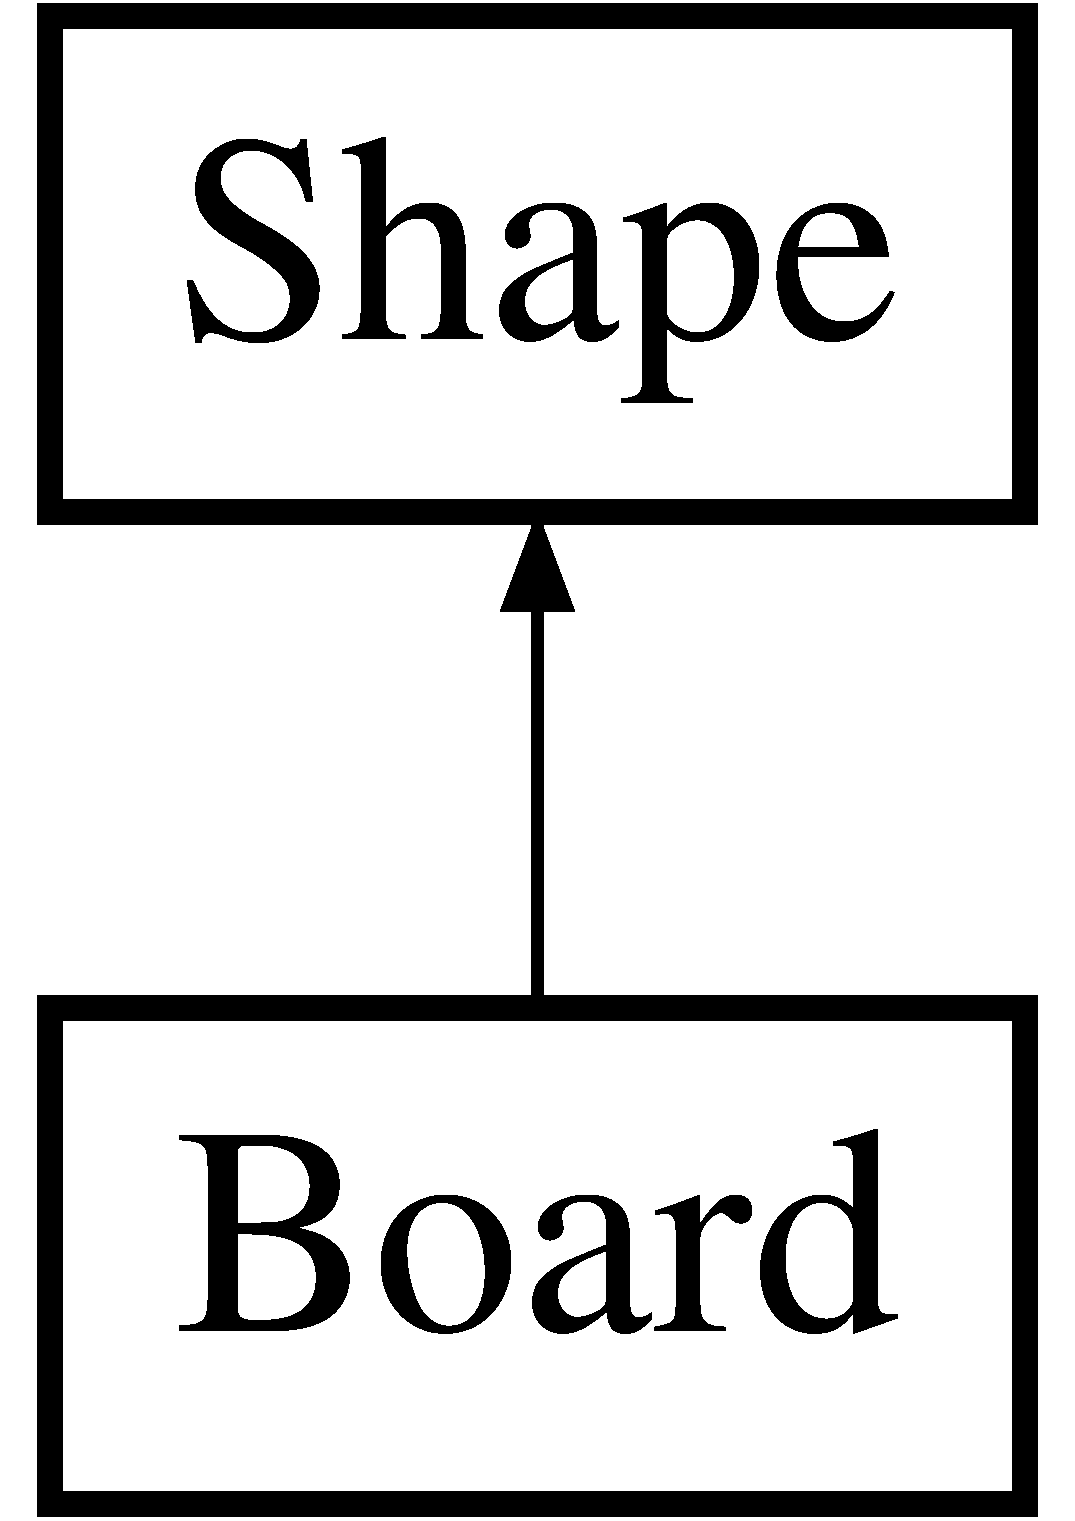
\includegraphics[height=3.000000cm]{class_shape}
\end{center}
\end{figure}
\subsection*{Public Member Functions}
\begin{DoxyCompactItemize}
\item 
virtual \mbox{\hyperlink{class_shape_a935afc9e576015f967d90de56977167d}{$\sim$\+Shape}} ()
\item 
\mbox{\hyperlink{class_shape_aaa8d87171e65e0d8ba3c5459978992a7}{Shape}} ()
\item 
\mbox{\hyperlink{class_shape_adb7c908a72cc99aee8c23ff0d4c6173a}{Shape}} (const unsigned int \&row, const unsigned int \&col)
\begin{DoxyCompactList}\small\item\em constructor for filled rectangle \end{DoxyCompactList}\item 
\mbox{\hyperlink{class_shape_a9004eb6a22e2f005aed9aac83aa7377b}{Shape}} (const std\+::vector$<$ std\+::vector$<$ bool $>$ $>$ \&bitmap)
\begin{DoxyCompactList}\small\item\em constructor for any shape \end{DoxyCompactList}\item 
virtual void \mbox{\hyperlink{class_shape_a285a0848e8bc19b0e76e2661d63bb1a1}{fill\+Bit\+Map}} (const unsigned int \&row, const unsigned int \&col)
\item 
virtual void \mbox{\hyperlink{class_shape_ae79ee483d0f48a426d1a544fd22fd8e5}{set\+Bit\+Map}} (const std\+::vector$<$ std\+::vector$<$ bool $>$ $>$ \&bitmap)
\item 
virtual int \mbox{\hyperlink{class_shape_a87f7e888ab40590dd3e4f73e13514152}{get\+Num\+Bit}} ()
\begin{DoxyCompactList}\small\item\em Count the number of unit squares inside the shape. \end{DoxyCompactList}\item 
virtual void \mbox{\hyperlink{class_shape_af3b265335667167ced81b3226b07dcb0}{set\+Bit}} (const int \&i, const int \&j, const bool \&k)
\begin{DoxyCompactList}\small\item\em set bit at specific position \end{DoxyCompactList}\item 
virtual bool \mbox{\hyperlink{class_shape_ab486d732a49d49cbbc4fadf1f23c379e}{get\+Bit}} (const int \&i, const int \&j) const
\begin{DoxyCompactList}\small\item\em get bit at specific position \end{DoxyCompactList}\item 
virtual int \mbox{\hyperlink{class_shape_a7f6887a6b1b1dfa6b7471edb4a582731}{get\+Col\+Num}} () const
\begin{DoxyCompactList}\small\item\em Get the number of columns of the shape. \end{DoxyCompactList}\item 
virtual int \mbox{\hyperlink{class_shape_a849c13a51a231c2ecb364efc3ff3f1ae}{get\+Row\+Num}} () const
\begin{DoxyCompactList}\small\item\em Get the number of rows of the shape. \end{DoxyCompactList}\item 
virtual void \mbox{\hyperlink{class_shape_a7f336c18e4bbd3035542037862d0eec7}{del}} ()
\end{DoxyCompactItemize}


\subsection{Detailed Description}
A bitmap representing shape. 

\subsection{Constructor \& Destructor Documentation}
\mbox{\Hypertarget{class_shape_a935afc9e576015f967d90de56977167d}\label{class_shape_a935afc9e576015f967d90de56977167d}} 
\index{Shape@{Shape}!````~Shape@{$\sim$\+Shape}}
\index{````~Shape@{$\sim$\+Shape}!Shape@{Shape}}
\subsubsection{\texorpdfstring{$\sim$\+Shape()}{~Shape()}}
{\footnotesize\ttfamily Shape\+::$\sim$\+Shape (\begin{DoxyParamCaption}{ }\end{DoxyParamCaption})\hspace{0.3cm}{\ttfamily [virtual]}}

\mbox{\Hypertarget{class_shape_aaa8d87171e65e0d8ba3c5459978992a7}\label{class_shape_aaa8d87171e65e0d8ba3c5459978992a7}} 
\index{Shape@{Shape}!Shape@{Shape}}
\index{Shape@{Shape}!Shape@{Shape}}
\subsubsection{\texorpdfstring{Shape()}{Shape()}\hspace{0.1cm}{\footnotesize\ttfamily [1/3]}}
{\footnotesize\ttfamily Shape\+::\+Shape (\begin{DoxyParamCaption}{ }\end{DoxyParamCaption})}

\mbox{\Hypertarget{class_shape_adb7c908a72cc99aee8c23ff0d4c6173a}\label{class_shape_adb7c908a72cc99aee8c23ff0d4c6173a}} 
\index{Shape@{Shape}!Shape@{Shape}}
\index{Shape@{Shape}!Shape@{Shape}}
\subsubsection{\texorpdfstring{Shape()}{Shape()}\hspace{0.1cm}{\footnotesize\ttfamily [2/3]}}
{\footnotesize\ttfamily Shape\+::\+Shape (\begin{DoxyParamCaption}\item[{const unsigned int \&}]{row,  }\item[{const unsigned int \&}]{col }\end{DoxyParamCaption})}



constructor for filled rectangle 


\begin{DoxyParams}{Parameters}
{\em row} & The number of rows of the rectangle \\
\hline
{\em col} & The number of columns of the rectangle \\
\hline
\end{DoxyParams}
\mbox{\Hypertarget{class_shape_a9004eb6a22e2f005aed9aac83aa7377b}\label{class_shape_a9004eb6a22e2f005aed9aac83aa7377b}} 
\index{Shape@{Shape}!Shape@{Shape}}
\index{Shape@{Shape}!Shape@{Shape}}
\subsubsection{\texorpdfstring{Shape()}{Shape()}\hspace{0.1cm}{\footnotesize\ttfamily [3/3]}}
{\footnotesize\ttfamily Shape\+::\+Shape (\begin{DoxyParamCaption}\item[{const std\+::vector$<$ std\+::vector$<$ bool $>$ $>$ \&}]{bitmap }\end{DoxyParamCaption})}



constructor for any shape 


\begin{DoxyParams}{Parameters}
{\em bitmap} & The bitmap representing the shape. \\
\hline
\end{DoxyParams}
\begin{DoxySeeAlso}{See also}
\mbox{\hyperlink{class_shape_ae79ee483d0f48a426d1a544fd22fd8e5}{set\+Bit\+Map()}} 
\end{DoxySeeAlso}


\subsection{Member Function Documentation}
\mbox{\Hypertarget{class_shape_a7f336c18e4bbd3035542037862d0eec7}\label{class_shape_a7f336c18e4bbd3035542037862d0eec7}} 
\index{Shape@{Shape}!del@{del}}
\index{del@{del}!Shape@{Shape}}
\subsubsection{\texorpdfstring{del()}{del()}}
{\footnotesize\ttfamily void Shape\+::del (\begin{DoxyParamCaption}{ }\end{DoxyParamCaption})\hspace{0.3cm}{\ttfamily [virtual]}}

\mbox{\Hypertarget{class_shape_a285a0848e8bc19b0e76e2661d63bb1a1}\label{class_shape_a285a0848e8bc19b0e76e2661d63bb1a1}} 
\index{Shape@{Shape}!fill\+Bit\+Map@{fill\+Bit\+Map}}
\index{fill\+Bit\+Map@{fill\+Bit\+Map}!Shape@{Shape}}
\subsubsection{\texorpdfstring{fill\+Bit\+Map()}{fillBitMap()}}
{\footnotesize\ttfamily void Shape\+::fill\+Bit\+Map (\begin{DoxyParamCaption}\item[{const unsigned int \&}]{row,  }\item[{const unsigned int \&}]{col }\end{DoxyParamCaption})\hspace{0.3cm}{\ttfamily [virtual]}}

\mbox{\Hypertarget{class_shape_ab486d732a49d49cbbc4fadf1f23c379e}\label{class_shape_ab486d732a49d49cbbc4fadf1f23c379e}} 
\index{Shape@{Shape}!get\+Bit@{get\+Bit}}
\index{get\+Bit@{get\+Bit}!Shape@{Shape}}
\subsubsection{\texorpdfstring{get\+Bit()}{getBit()}}
{\footnotesize\ttfamily bool Shape\+::get\+Bit (\begin{DoxyParamCaption}\item[{const int \&}]{i,  }\item[{const int \&}]{j }\end{DoxyParamCaption}) const\hspace{0.3cm}{\ttfamily [virtual]}}



get bit at specific position 


\begin{DoxyParams}{Parameters}
{\em i} & The row containing the bit \\
\hline
{\em j} & The column containing the bit \\
\hline
\end{DoxyParams}
\begin{DoxySeeAlso}{See also}
\mbox{\hyperlink{class_shape_af3b265335667167ced81b3226b07dcb0}{set\+Bit()}} 
\end{DoxySeeAlso}
\mbox{\Hypertarget{class_shape_a7f6887a6b1b1dfa6b7471edb4a582731}\label{class_shape_a7f6887a6b1b1dfa6b7471edb4a582731}} 
\index{Shape@{Shape}!get\+Col\+Num@{get\+Col\+Num}}
\index{get\+Col\+Num@{get\+Col\+Num}!Shape@{Shape}}
\subsubsection{\texorpdfstring{get\+Col\+Num()}{getColNum()}}
{\footnotesize\ttfamily int Shape\+::get\+Col\+Num (\begin{DoxyParamCaption}{ }\end{DoxyParamCaption}) const\hspace{0.3cm}{\ttfamily [virtual]}}



Get the number of columns of the shape. 

\begin{DoxySeeAlso}{See also}
\mbox{\hyperlink{class_shape_a849c13a51a231c2ecb364efc3ff3f1ae}{get\+Row\+Num()}} 
\end{DoxySeeAlso}
\mbox{\Hypertarget{class_shape_a87f7e888ab40590dd3e4f73e13514152}\label{class_shape_a87f7e888ab40590dd3e4f73e13514152}} 
\index{Shape@{Shape}!get\+Num\+Bit@{get\+Num\+Bit}}
\index{get\+Num\+Bit@{get\+Num\+Bit}!Shape@{Shape}}
\subsubsection{\texorpdfstring{get\+Num\+Bit()}{getNumBit()}}
{\footnotesize\ttfamily int Shape\+::get\+Num\+Bit (\begin{DoxyParamCaption}{ }\end{DoxyParamCaption})\hspace{0.3cm}{\ttfamily [virtual]}}



Count the number of unit squares inside the shape. 

\mbox{\Hypertarget{class_shape_a849c13a51a231c2ecb364efc3ff3f1ae}\label{class_shape_a849c13a51a231c2ecb364efc3ff3f1ae}} 
\index{Shape@{Shape}!get\+Row\+Num@{get\+Row\+Num}}
\index{get\+Row\+Num@{get\+Row\+Num}!Shape@{Shape}}
\subsubsection{\texorpdfstring{get\+Row\+Num()}{getRowNum()}}
{\footnotesize\ttfamily int Shape\+::get\+Row\+Num (\begin{DoxyParamCaption}{ }\end{DoxyParamCaption}) const\hspace{0.3cm}{\ttfamily [virtual]}}



Get the number of rows of the shape. 

\begin{DoxySeeAlso}{See also}
\mbox{\hyperlink{class_shape_a7f6887a6b1b1dfa6b7471edb4a582731}{get\+Col\+Num()}} 
\end{DoxySeeAlso}
\mbox{\Hypertarget{class_shape_af3b265335667167ced81b3226b07dcb0}\label{class_shape_af3b265335667167ced81b3226b07dcb0}} 
\index{Shape@{Shape}!set\+Bit@{set\+Bit}}
\index{set\+Bit@{set\+Bit}!Shape@{Shape}}
\subsubsection{\texorpdfstring{set\+Bit()}{setBit()}}
{\footnotesize\ttfamily void Shape\+::set\+Bit (\begin{DoxyParamCaption}\item[{const int \&}]{i,  }\item[{const int \&}]{j,  }\item[{const bool \&}]{k }\end{DoxyParamCaption})\hspace{0.3cm}{\ttfamily [virtual]}}



set bit at specific position 


\begin{DoxyParams}{Parameters}
{\em i} & The row containing the bit \\
\hline
{\em j} & The column containing the bit \\
\hline
{\em k} & New value of the bit \\
\hline
\end{DoxyParams}
\begin{DoxySeeAlso}{See also}
\mbox{\hyperlink{class_shape_ab486d732a49d49cbbc4fadf1f23c379e}{get\+Bit()}} 
\end{DoxySeeAlso}
\mbox{\Hypertarget{class_shape_ae79ee483d0f48a426d1a544fd22fd8e5}\label{class_shape_ae79ee483d0f48a426d1a544fd22fd8e5}} 
\index{Shape@{Shape}!set\+Bit\+Map@{set\+Bit\+Map}}
\index{set\+Bit\+Map@{set\+Bit\+Map}!Shape@{Shape}}
\subsubsection{\texorpdfstring{set\+Bit\+Map()}{setBitMap()}}
{\footnotesize\ttfamily void Shape\+::set\+Bit\+Map (\begin{DoxyParamCaption}\item[{const std\+::vector$<$ std\+::vector$<$ bool $>$ $>$ \&}]{bitmap }\end{DoxyParamCaption})\hspace{0.3cm}{\ttfamily [virtual]}}



The documentation for this class was generated from the following files\+:\begin{DoxyCompactItemize}
\item 
\mbox{\hyperlink{shape_8h}{shape.\+h}}\item 
\mbox{\hyperlink{shape_8cpp}{shape.\+cpp}}\end{DoxyCompactItemize}

\chapter{File Documentation}
\hypertarget{board_8h}{}\section{board.\+h File Reference}
\label{board_8h}\index{board.\+h@{board.\+h}}


Include file for \mbox{\hyperlink{class_board}{Board}} handling.  


{\ttfamily \#include \char`\"{}visible\+\_\+shape.\+h\char`\"{}}\newline
{\ttfamily \#include \char`\"{}encrypted\+\_\+num.\+h\char`\"{}}\newline
\subsection*{Classes}
\begin{DoxyCompactItemize}
\item 
class \mbox{\hyperlink{class_board}{Board}}
\begin{DoxyCompactList}\small\item\em The board where pieces are placed. \end{DoxyCompactList}\end{DoxyCompactItemize}


\subsection{Detailed Description}
Include file for \mbox{\hyperlink{class_board}{Board}} handling. 


\hypertarget{button_8h}{}\section{button.\+h File Reference}
\label{button_8h}\index{button.\+h@{button.\+h}}


Include file for \mbox{\hyperlink{class_button}{Button}} handling.  


{\ttfamily \#include \char`\"{}image.\+h\char`\"{}}\newline
{\ttfamily \#include \char`\"{}font.\+h\char`\"{}}\newline
\subsection*{Classes}
\begin{DoxyCompactItemize}
\item 
class \mbox{\hyperlink{class_button}{Button}}
\begin{DoxyCompactList}\small\item\em A class that defines button including icon and text. \end{DoxyCompactList}\end{DoxyCompactItemize}


\subsection{Detailed Description}
Include file for \mbox{\hyperlink{class_button}{Button}} handling. 


\hypertarget{color_8h}{}\section{color.\+h File Reference}
\label{color_8h}\index{color.\+h@{color.\+h}}


Include file for \mbox{\hyperlink{class_color}{Color}} handling.  


\subsection*{Classes}
\begin{DoxyCompactItemize}
\item 
class \mbox{\hyperlink{class_color}{Color}}
\begin{DoxyCompactList}\small\item\em A class that defines color. \end{DoxyCompactList}\end{DoxyCompactItemize}


\subsection{Detailed Description}
Include file for \mbox{\hyperlink{class_color}{Color}} handling. 


\hypertarget{main_8cpp}{}\section{main.\+cpp File Reference}
\label{main_8cpp}\index{main.\+cpp@{main.\+cpp}}


This file starts the game.  


{\ttfamily \#include \char`\"{}S\+D\+L\+\_\+utils.\+h\char`\"{}}\newline
{\ttfamily \#include \char`\"{}board\+\_\+surface.\+h\char`\"{}}\newline
{\ttfamily \#include \char`\"{}menu\+\_\+surface.\+h\char`\"{}}\newline
{\ttfamily \#include \char`\"{}visible\+\_\+encrypted\+\_\+num\+\_\+surface.\+h\char`\"{}}\newline
{\ttfamily \#include \char`\"{}visible\+\_\+shape\+\_\+surface.\+h\char`\"{}}\newline
{\ttfamily \#include $<$time.\+h$>$}\newline
\subsection*{Classes}
\begin{DoxyCompactItemize}
\item 
class \mbox{\hyperlink{class_game1010}{Game1010}}
\begin{DoxyCompactList}\small\item\em The game itself. \end{DoxyCompactList}\end{DoxyCompactItemize}
\subsection*{Functions}
\begin{DoxyCompactItemize}
\item 
int \mbox{\hyperlink{main_8cpp_a3c04138a5bfe5d72780bb7e82a18e627}{main}} (int argc, char $\ast$$\ast$argv)
\end{DoxyCompactItemize}


\subsection{Detailed Description}
This file starts the game. 

\begin{DoxyAuthor}{Author}
Nguyen Minh Tan 
\end{DoxyAuthor}
\begin{DoxyVersion}{Version}
1.\+5.\+0 
\end{DoxyVersion}
\begin{DoxyDate}{Date}
05/05/2019 
\end{DoxyDate}
\begin{DoxyPrecond}{Precondition}
Add linker options\+: -\/lmingw32 -\/l\+S\+D\+L2main -\/l\+S\+D\+L2 -\/l\+S\+D\+L2\+\_\+image -\/l\+S\+D\+L2\+\_\+ttf -\/l\+S\+D\+L2\+\_\+mixer. Then search directories\+: Compiler for include\textbackslash{} folder and Linker for lib\textbackslash{} folder. 
\end{DoxyPrecond}


\subsection{Function Documentation}
\mbox{\Hypertarget{main_8cpp_a3c04138a5bfe5d72780bb7e82a18e627}\label{main_8cpp_a3c04138a5bfe5d72780bb7e82a18e627}} 
\index{main.\+cpp@{main.\+cpp}!main@{main}}
\index{main@{main}!main.\+cpp@{main.\+cpp}}
\subsubsection{\texorpdfstring{main()}{main()}}
{\footnotesize\ttfamily int main (\begin{DoxyParamCaption}\item[{int}]{argc,  }\item[{char $\ast$$\ast$}]{argv }\end{DoxyParamCaption})}


\hypertarget{menu_8h}{}\section{menu.\+h File Reference}
\label{menu_8h}\index{menu.\+h@{menu.\+h}}


Include file for \mbox{\hyperlink{class_menu}{Menu}} handling.  


{\ttfamily \#include \char`\"{}button.\+h\char`\"{}}\newline
{\ttfamily \#include $<$vector$>$}\newline
\subsection*{Classes}
\begin{DoxyCompactItemize}
\item 
class \mbox{\hyperlink{class_menu}{Menu}}
\begin{DoxyCompactList}\small\item\em A class that defines menu consisting of buttons. \end{DoxyCompactList}\end{DoxyCompactItemize}


\subsection{Detailed Description}
Include file for \mbox{\hyperlink{class_menu}{Menu}} handling. 


\hypertarget{score_8h}{}\section{score.\+h File Reference}
\label{score_8h}\index{score.\+h@{score.\+h}}


Include file for \mbox{\hyperlink{class_score}{Score}} handling.  


{\ttfamily \#include $<$fstream$>$}\newline
{\ttfamily \#include $<$stdlib.\+h$>$}\newline
{\ttfamily \#include $<$time.\+h$>$}\newline
{\ttfamily \#include $<$vector$>$}\newline
\subsection*{Classes}
\begin{DoxyCompactItemize}
\item 
class \mbox{\hyperlink{class_score}{Score}}
\begin{DoxyCompactList}\small\item\em A class that defines score. \end{DoxyCompactList}\end{DoxyCompactItemize}


\subsection{Detailed Description}
Include file for \mbox{\hyperlink{class_score}{Score}} handling. 


\hypertarget{_s_d_l__utils_8h}{}\section{S\+D\+L\+\_\+utils.\+h File Reference}
\label{_s_d_l__utils_8h}\index{S\+D\+L\+\_\+utils.\+h@{S\+D\+L\+\_\+utils.\+h}}


Include file for creating window and rendering textures.  


{\ttfamily \#include \char`\"{}isurface.\+h\char`\"{}}\newline
{\ttfamily \#include $<$S\+D\+L.\+h$>$}\newline
{\ttfamily \#include $<$S\+D\+L\+\_\+image.\+h$>$}\newline
{\ttfamily \#include $<$S\+D\+L\+\_\+ttf.\+h$>$}\newline
{\ttfamily \#include $<$S\+D\+L\+\_\+mixer.\+h$>$}\newline
{\ttfamily \#include $<$iostream$>$}\newline
{\ttfamily \#include $<$cstdlib$>$}\newline
\subsection*{Classes}
\begin{DoxyCompactItemize}
\item 
class \mbox{\hyperlink{class_s_d_l_utils}{S\+D\+L\+Utils}}
\begin{DoxyCompactList}\small\item\em A window displaying textures. \end{DoxyCompactList}\end{DoxyCompactItemize}


\subsection{Detailed Description}
Include file for creating window and rendering textures. 

\begin{DoxyPrecond}{Precondition}
Add linker options\+: -\/lmingw32 -\/l\+S\+D\+L2main -\/l\+S\+D\+L2 -\/l\+S\+D\+L2\+\_\+image -\/l\+S\+D\+L2\+\_\+ttf -\/l\+S\+D\+L2\+\_\+mixer. Then search directories\+: Compiler for include\textbackslash{} folder and Linker for lib\textbackslash{} folder. 
\end{DoxyPrecond}

\hypertarget{shape_8h}{}\section{shape.\+h File Reference}
\label{shape_8h}\index{shape.\+h@{shape.\+h}}


Include file for \mbox{\hyperlink{class_shape}{Shape}} handling.  


{\ttfamily \#include $<$vector$>$}\newline
\subsection*{Classes}
\begin{DoxyCompactItemize}
\item 
class \mbox{\hyperlink{class_shape}{Shape}}
\begin{DoxyCompactList}\small\item\em A bitmap representing shape. \end{DoxyCompactList}\end{DoxyCompactItemize}


\subsection{Detailed Description}
Include file for \mbox{\hyperlink{class_shape}{Shape}} handling. 


%--- End generated contents ---

% Index
\backmatter
\newpage
\phantomsection
\clearemptydoublepage
\addcontentsline{toc}{chapter}{Index}
\printindex

\end{document}
